\documentclass[a4paper,12pt]{article}
\usepackage[utf8]{inputenc}
\usepackage{listings}
\usepackage{amsmath, amssymb} % For math symbols and equations
\usepackage{geometry} % For page margin settings
\geometry{margin=1in} % Set page margins
\usepackage{graphicx} % For including images
\title{Computerized Simulation \\
Exercise No. 1}
\author{name : Seyed Mohammad Ghoreishy \\ teacher : Seyed Amirhossein Tabatabaei }
\date{Date: 1403.08.21}
\begin{document}
\maketitle
\tableofcontents 
\newpage
\section{Exercise 1}
\subsection{Chapter 2-Exercises 1}
Solution for 2.1
\begin{figure}[h!]
    \centering
    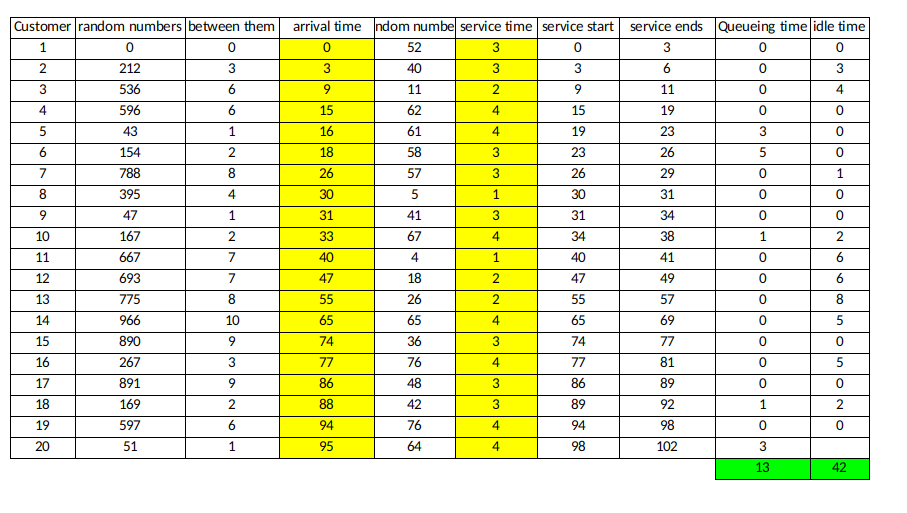
\includegraphics[width=1\textwidth]{./Screenshots/Exercise1.1.xlsx.png} 
\end{figure} \\
Explanation of file structure and cells
\begin{itemize}
    \item Customer from 1 to 20 
    \item random numbers : TRUNC(RAND()*1000)
    \item arrival time   : Arrival time plus the time between two arrivals
    \item service time   : IF(E5\textless11,1,IF(E5\textless31,2,IF(E5\textless61,3,IF(E5\textless86,4,IF(E5\textless96,5,6)))))
    \item service start  : If the arrival time was after the previous finish: the arrival time, otherwise, the previous finish time
    \item service ends   : start time plus service time 
    \item Queueing time  : Difference between arrival time and start time
    \item idle time      : The difference between the previous end and the next start
\end{itemize}
Average waiting time : \(\frac{51}{20} \) \\
The possibility of idle : \(\frac{15}{88} \) \\
It can be seen that the duration of unemployment is opposite to the waiting time
And in the data where the service time is high, the waiting time of customers increases
\newpage
\subsection{Chapter 2-Exercises 2}
Solution for 2.2 \\
\begin{figure}[h!]
    \centering
    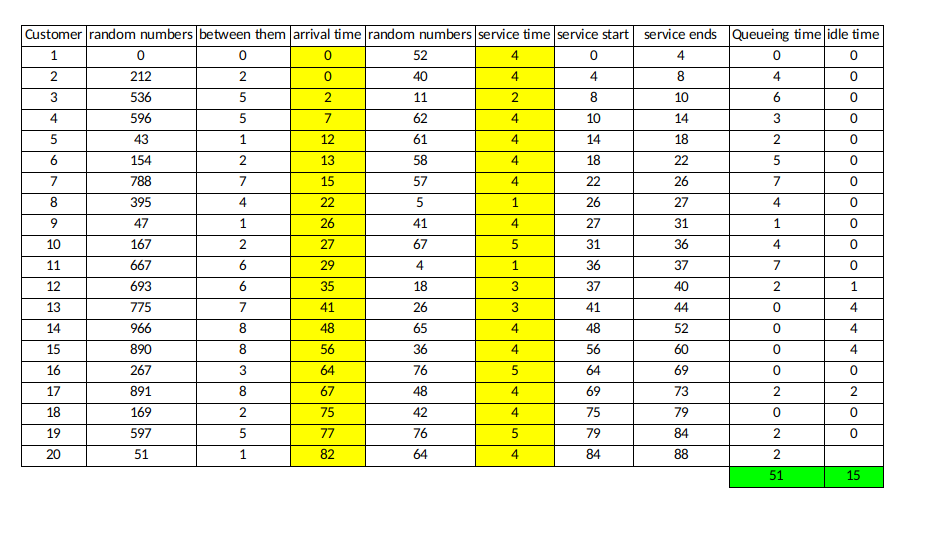
\includegraphics[width=1\textwidth]{./Screenshots/Exercise1.2.xlsx.png} 
\end{figure}
Average waiting time : \(\frac{13}{20} \) \\
The possibility of idle : \(\frac{42}{102} \) \\
In this example, it shows that if we change the servicing on the same previous data
Queueing time is lower, but idle time is higher
\newpage
\subsection{Chapter 2-Exercises 3}
Solution for 2.3 
\begin{figure}[h!]
    \centering
    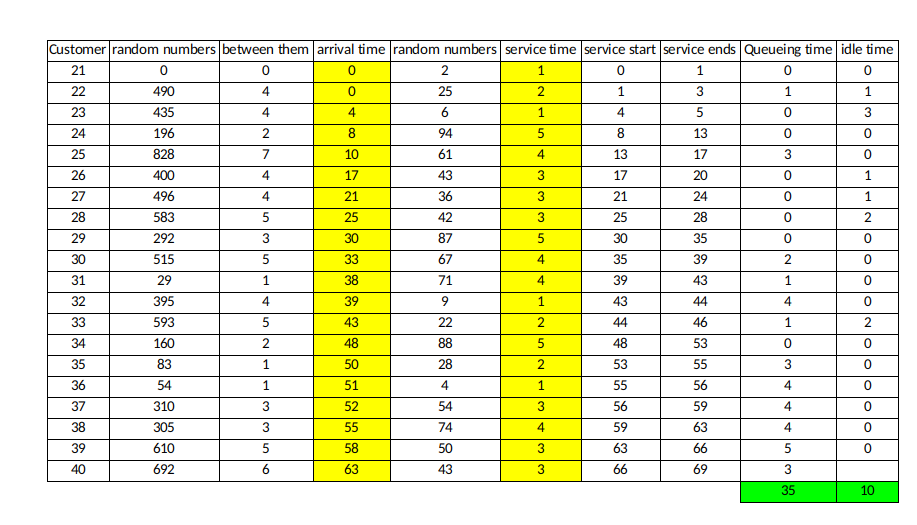
\includegraphics[width=1\textwidth]{./Screenshots/Exercise1.3.xlsx.png} 
\end{figure} \\
It shows by comparing the current results and results the inside of the book \\
Both of our times have decreased, which is due to the creation of random data \\
Because the sample size is very small, so two samples have a lot of variance
\newpage
\subsection{Chapter 2-Exercises 5}
in file Exercise1.4.xlsx has three sheets, in the first sheet, the book's problem is simulated, \\
and in the second sheet, the same random numbers are simulated with a new distribution. \\
And in the third sheet where there is a compilation of data, it can be seen that the Queueing time of customers have increased, but the average idle time service has decreased.
\\ for example:
\begin{figure}[h!]
    \centering
    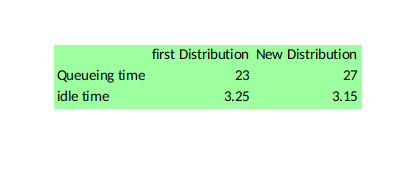
\includegraphics[width=0.6\textwidth]{./Screenshots/Exercise1.4.xlsx.png} 
\end{figure} \\
\newpage

\subsection{Chapter 2-Exercises 14}
in file Exercise1.5.xlsx has three sheets
 the third sheet where there is a results of data,Customer waiting time has increased, but the unemployment of taxis will be close to zero
\\ for example:
\begin{figure}[h!]
    \centering
    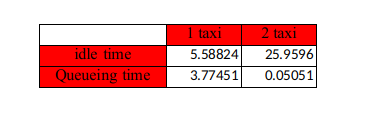
\includegraphics[width=0.6\textwidth]{./Screenshots/Exercise1.5.xlsx.png} 
\end{figure} \\
\newpage
\subsection{Chapter 2-Exercises 16}
\begin{figure}[h!]
    \centering
    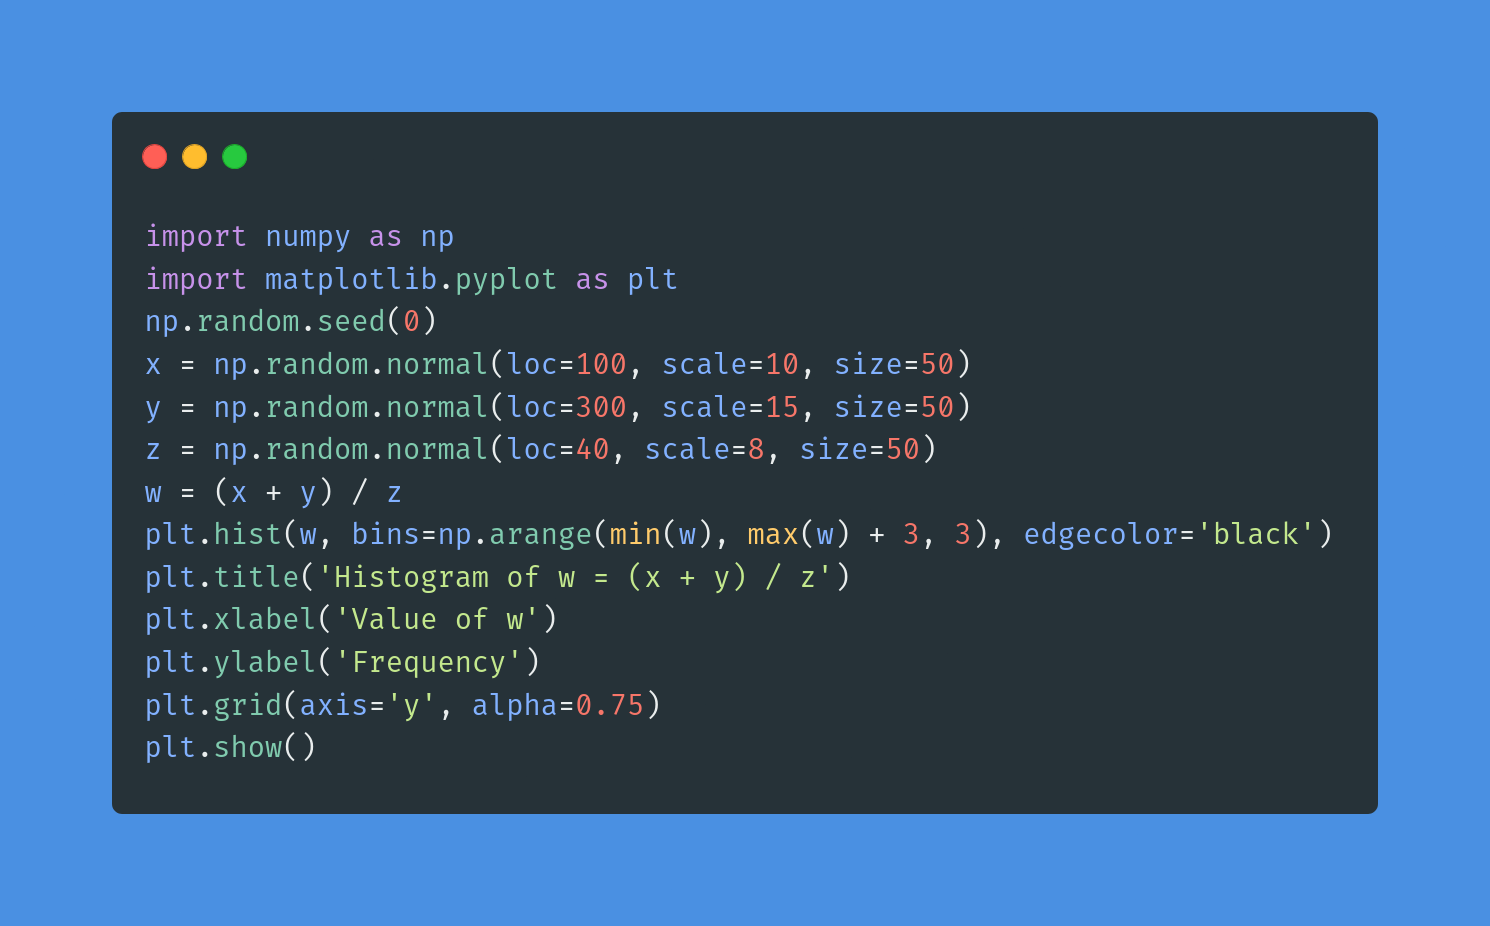
\includegraphics[width=0.8\textwidth]{./Screenshots/Exercise1.6.py.png} 
\end{figure} \\
\begin{figure}[h!]
    \centering
    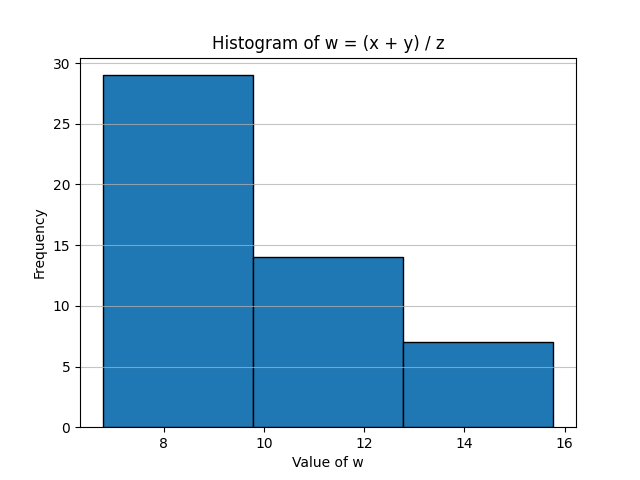
\includegraphics[width=0.8\textwidth]{./Screenshots/Exercise1.6.png} 
\end{figure} \\
\newpage
\subsection{Chapter 2-Exercises 21}
\begin{figure}[h!]
    \centering
    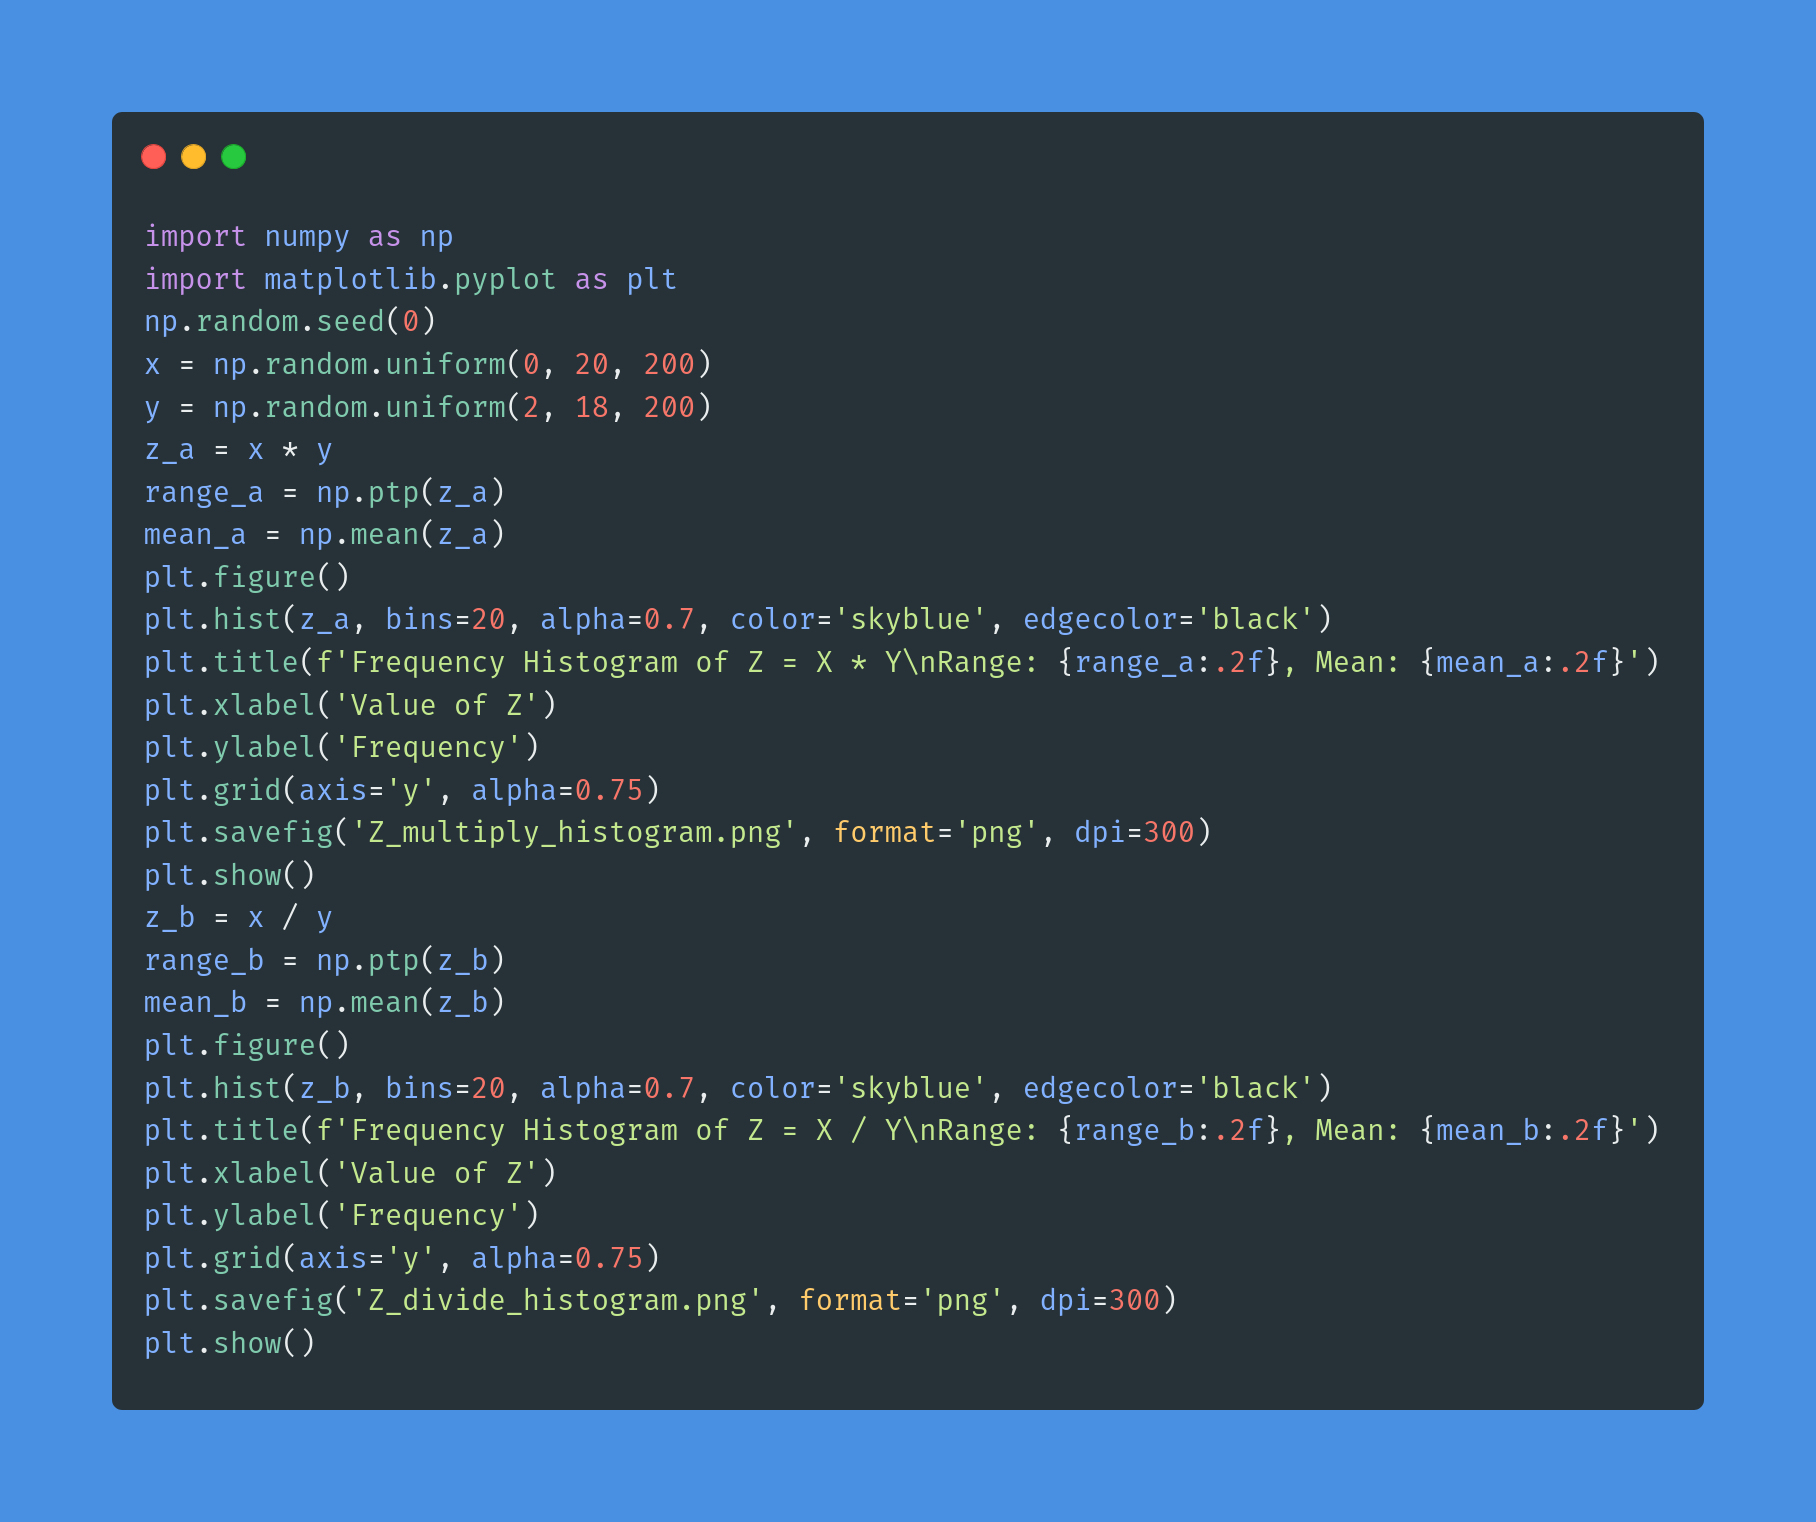
\includegraphics[width=0.8\textwidth]{./Screenshots/Exercise1.7.py.png} 
\end{figure} \\
\begin{figure}[h!]
    \centering
    \begin{minipage}{0.5\textwidth}
        \centering
        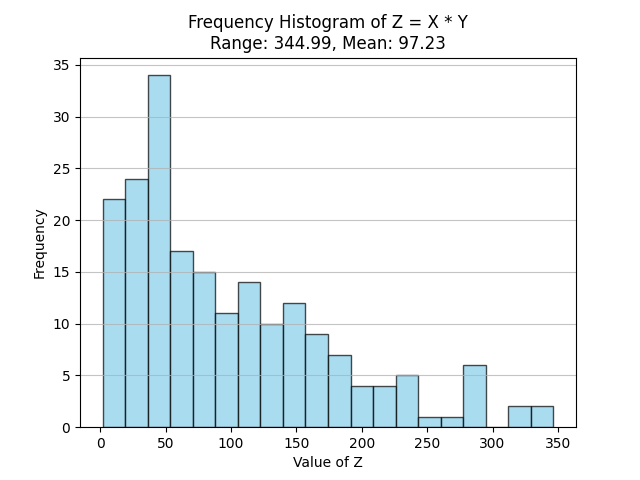
\includegraphics[width=\textwidth]{./Screenshots/Exercise1.7.1.png}
    \end{minipage}%
    \hfill
    \begin{minipage}{0.5\textwidth}
        \centering
        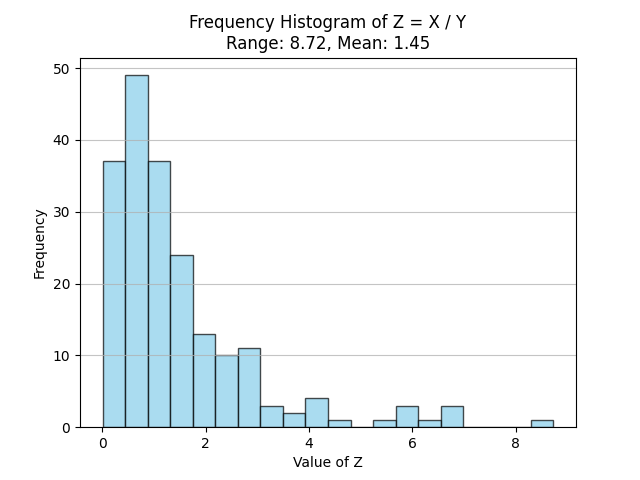
\includegraphics[width=\textwidth]{./Screenshots/Exercise1.7.2.png}
    \end{minipage}
\end{figure} \\

\newpage
\section{Exercise 2}
\subsection*{Part 1: \( U + 1 \)}
Since \( U \) has a uniform distribution on \( [0,1] \), its probability density function \( f_U(u) \) is :
\[
f_U(u) = 
\begin{cases} 
      1 & 0 \le u \le 1 \\
      0 & \text{otherwise}
\end{cases}
\]

Since \( U \) is uniformly distributed in \( [0, 1] \), the range of \( U + 1 \) will be \( [1, 2] \).

Define \( V = U + 1 \). Now, we want to determine the probability distribution of \( V \):

1. \textbf{Cumulative Distribution Function (CDF) of \( V \):}

   For \( v \in [1, 2] \):
   \[
   F_V(v) = P(V \le v) = P(U + 1 \le v) = P(U \le v - 1)
   \]
   
   Since \( U \) is uniform on \( [0, 1] \), the CDF of \( U \) is \( F_U(u) = u \). Therefore:
   \[
   F_V(v) = v - 1 \quad \text{for } v \in [1, 2]
   \]

2. \textbf{Probability Density Function (PDF) of \( V \):}
   \[
   f_V(v) = \frac{d}{dv} F_V(v) = \frac{d}{dv} (v - 1) = 1
   \]
   
   Therefore, \( V = U + 1 \) has a constant density over \( [1, 2] \), indicating a uniform distribution on \( [1, 2] \).

\subsection*{Part 2: \( U^2 \)}

Define \( W = U^2 \). If \( W \) were uniformly distributed, its PDF would be constant over its range \( [0, 1] \). Let’s calculate the CDF of \( W \) to find its PDF:

1. \textbf{Cumulative Distribution Function (CDF) of \( W \):}

   For \( w \in [0, 1] \):
   \[
   F_W(w) = P(W \le w) = P(U^2 \le w) = P(U \le \sqrt{w})
   \]
   
   Since \( U \) is uniform on \( [0, 1] \), we have \( F_U(u) = u \). Therefore:
   \[
   F_W(w) = \sqrt{w} \quad \text{for } w \in [0, 1]
   \]

2. \textbf{Probability Density Function (PDF) of \( W \):}

   Differentiating \( F_W(w) \) with respect to \( w \) gives us:
   \[
   f_W(w) = \frac{d}{dw} F_W(w) = \frac{d}{dw} (\sqrt{w}) = \frac{1}{2\sqrt{w}}
   \]
   
   Since \( f_W(w) = \frac{1}{2\sqrt{w}} \) is not constant over \( [0, 1] \), \( W = U^2 \) does not have a uniform distribution. Instead, this PDF indicates a higher probability density near zero.
\subsection*{Conclusion}
\begin{itemize}
    \item \( U + 1 \) has a uniform distribution on \( [1, 2] \).
    \item \( U^2 \) does not have a uniform distribution because its PDF is not constant on \( [0, 1] \).
\end{itemize}
\newpage

\section{Exercise 3}
To solve this problem, we can use the \textbf{Central Limit Theorem (CLT)}. The CLT states that, for a large number of independent and identically distributed random variables, the sum (or average) of these variables tends to follow a normal distribution, even if the original variables themselves do not follow a normal distribution.


Let \( X_1, X_2, \ldots, X_{50} \) be the service times for each of the 50 customers.Each \( X_i \) has mean \( E(X_i) = 2 \) and variance \( \text{Var}(X_i) = 1 \).
\\The total service time \( Y \) for 50 customers is:
  \[
  Y = \sum_{i=1}^{50} X_i
  \]

#### Step 1: Expected Value of \( Y \)
\[
E(Y) = \sum_{i=1}^{50} E(X_i) = 50 \times 2 = 100
\]

#### Step 2: Variance of \( Y \)

Since the \( X_i \) are independent, the variance of \( Y \) is the sum of the variances of \( X_i \):
\[
\text{Var}(Y) = \sum_{i=1}^{50} \text{Var}(X_i) = 50 \times 1 = 50
\]

The standard deviation of \( Y \) is therefore:
\[
\sigma_Y = \sqrt{\text{Var}(Y)} = \sqrt{50} \approx 7.07
\]

#### Step 3: Using the Central Limit Theorem to Approximate the Distribution of \( Y \)

By the Central Limit Theorem, for a sufficiently large \( n \) (here \( n = 50 \) is generally large enough), \( Y \) is approximately normally distributed with mean \( E(Y) = 100 \) and standard deviation \( \sigma_Y = 7.07 \):
\[
Y \sim N(100, 7.07^2)
\]

#### Step 4: Calculating \( P(90 < Y < 110) \)

We want to find \( P(90 < Y < 110) \). To do this, we standardize \( Y \) to convert it to the standard normal distribution.

1. Standardize 90:
   \[
   Z_1 = \frac{90 - 100}{7.07} \approx -1.41
   \]

2. Standardize 110:
   \[
   Z_2 = \frac{110 - 100}{7.07} \approx 1.41
   \]

Now, we need to find \( P(-1.41 < Z < 1.41) \), where \( Z \) follows a standard normal distribution.

Using a standard normal table or calculator:

\[
    P(90 < Y < 110) = P(-1.41 < Z < 1.41) = P(Z < 1.41) - P(Z < -1.41) \approx 0.9207 - 0.0793 = 0.8414
\]

\newpage
\section{Exercise 4}
In this problem, the probability of an error for each bit is \( p = 0.1 \) and the total number of bits in each packet is \( n = 1000 \). This follows a \textbf{binomial distribution} in which we want to find the probability of more than 120 errors.
\[
X \sim \text{Binomial}(n = 1000, p = 0.1)
\]

To approximate this probability, we can use the normal approximation to the binomial distribution, as \( n \) is large, and \( np \) and \( n(1 - p) \) are sufficiently large. According to the \textbf{Central Limit Theorem}, a binomial distribution with large parameters can be approximated by a normal distribution.

#### Step 1: Mean and Variance of the Binomial Distribution

For a binomial distribution \( \text{Binomial}(n, p) \), we have:
\[
\mu = np = 1000 \times 0.1 = 100
\]
\[
\sigma^2 = np(1 - p) = 1000 \times 0.1 \times 0.9 = 90
\]
Therefore, the standard deviation \( \sigma \) is:
\[
\sigma = \sqrt{90} \approx 9.49
\]

#### Step 2: Normal Approximation to Find \( P(X > 120) \)

Using the normal approximation:
\[
X \sim N(100, 9.49^2)
\]

We want to find \( P(X > 120) \). To do this, we first convert \( X = 120 \) to the standard normal variable \( Z \).

#### Step 3: Calculating \( Z \)

Standardizing:
\[
Z = \frac{120 - \mu}{\sigma} = \frac{120 - 100}{9.49} \approx 2.11
\]

#### Step 4: Finding \( P(Z > 2.11) \)

Using a standard normal table or calculator:
\[
P(Z > 2.11) \approx 0.0174
\]
\newpage
\section{Exercise 5}
To generate random points uniformly distributed within an ellipse, we can follow these steps:

\textbf{1.Ellipse Equation:}
   \[
   \frac{x^2}{a^2} + \frac{y^2}{b^2} \leq 1
   \]
   Any point \( (x, y) \) that satisfies this inequality lies within the ellipse.

\textbf{2. Uniform Sampling within the Ellipse:}
\\To generate points uniformly within the ellipse, we can start by generating points in a unit circle, then scale them to fit the ellipse.

\textbf{3. Steps for Sampling:}
   \\- Step 1: Generate a random angle \( \theta \) uniformly from \( [0, 2\pi] \).
   \\- Step 2: Generate a radius \( r \) uniformly from \( [0, 1] \) and take its square root. This ensures that the points are uniformly distributed within the unit circle.
   \\- Step 3: Calculate the coordinates in the unit circle as:
     \[
     x_{\text{circle}} = r \cos \theta, \quad y_{\text{circle}} = r \sin \theta
     \]
   - Step 4: Map these points to the ellipse by scaling them with \( a \) and \( b \):
     \[
     x = a \cdot x_{\text{circle}}, \quad y = b \cdot y_{\text{circle}}
     \]

\begin{figure}[h!]
    \centering
    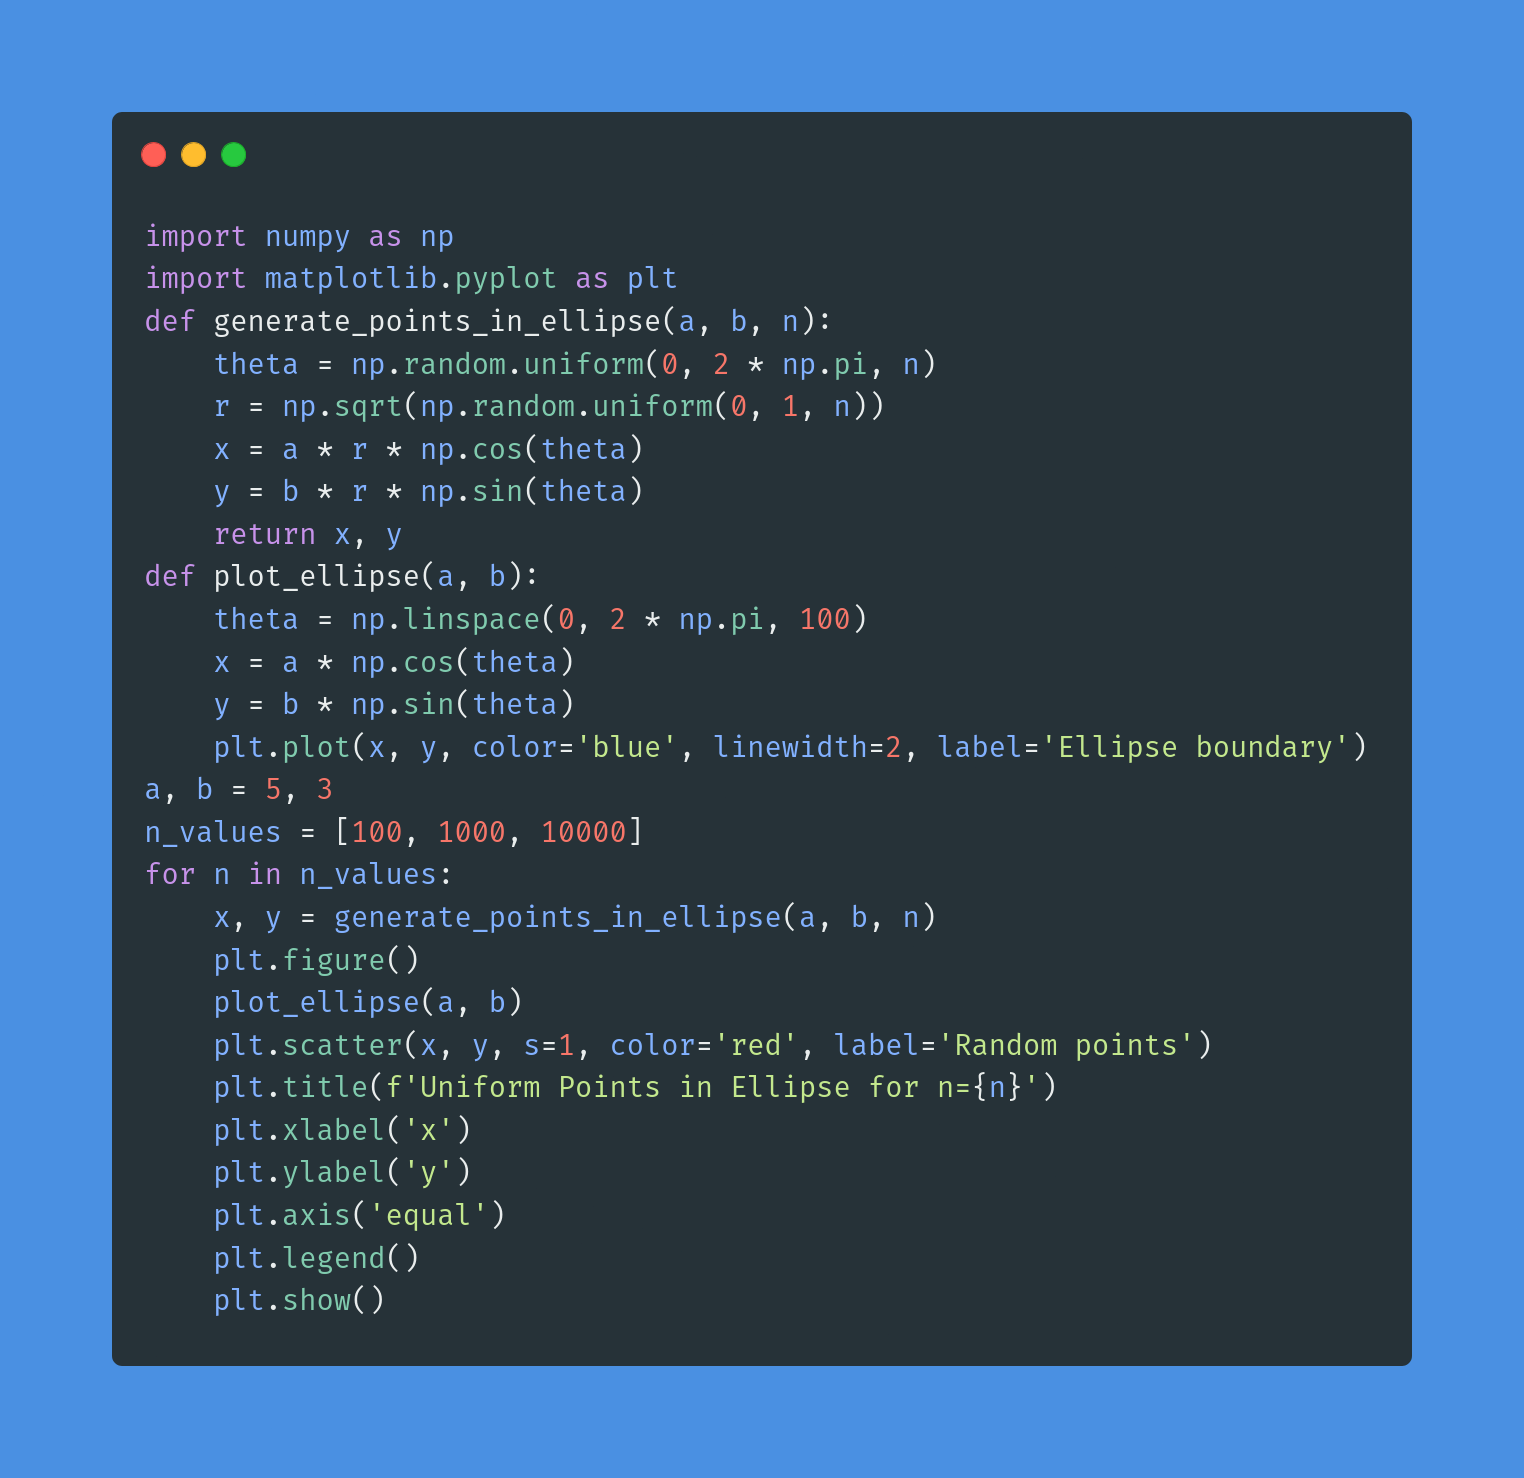
\includegraphics[width=0.5\textwidth]{./Screenshots/Exercise5.py.png} 
\end{figure} \\
\begin{figure}[h!]
    \centering
    \begin{minipage}{0.33\textwidth}
        \centering
        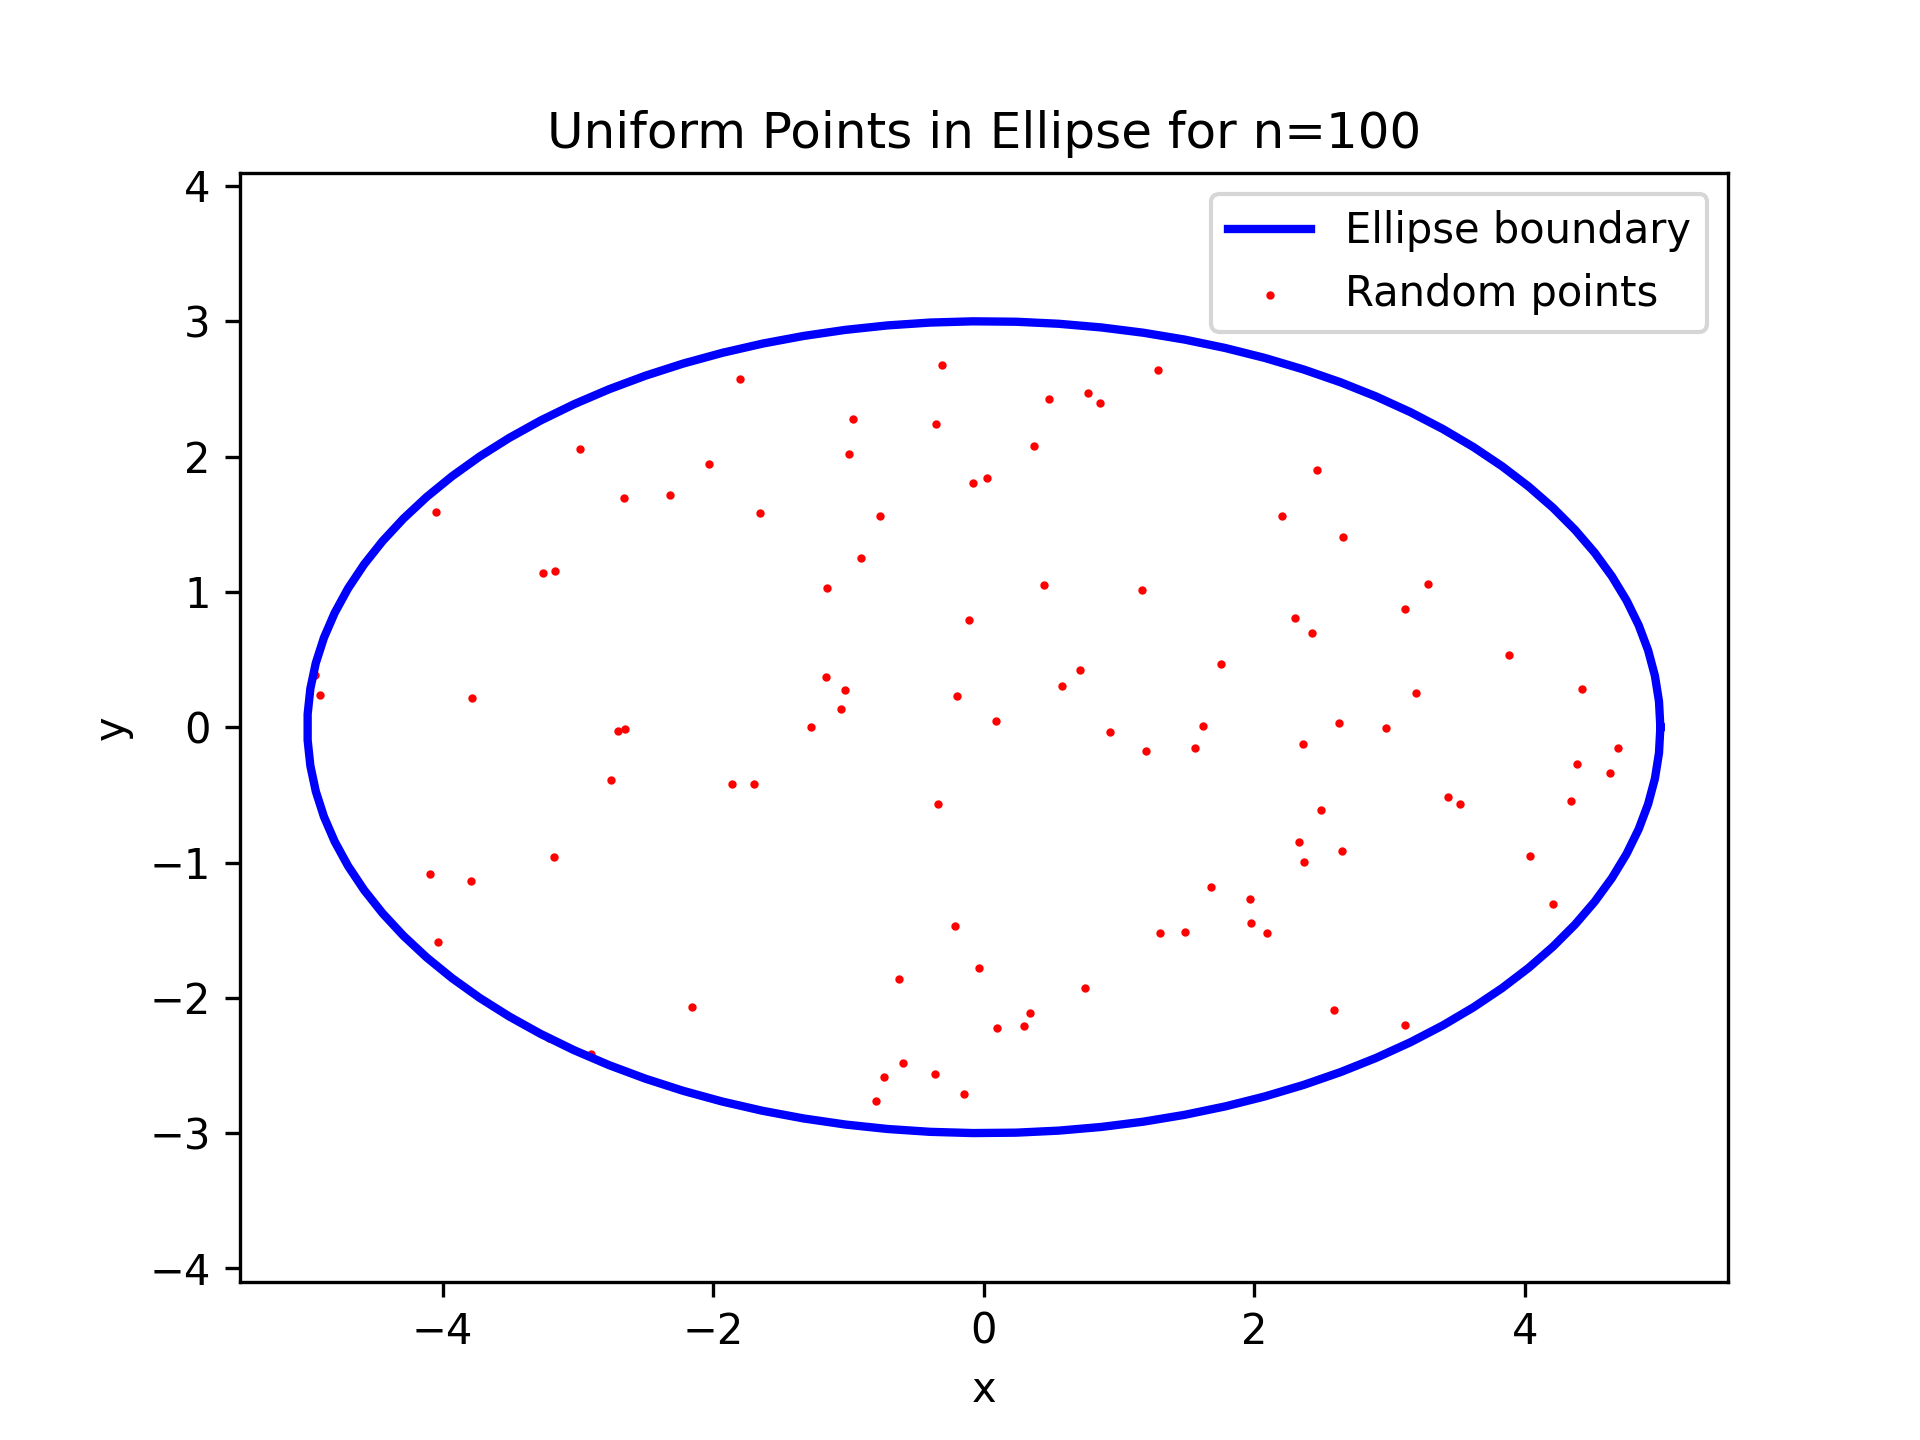
\includegraphics[width=\textwidth]{./Screenshots/Exercise5.1.png}
    \end{minipage}%
    \hfill
    \begin{minipage}{0.33\textwidth}
        \centering
        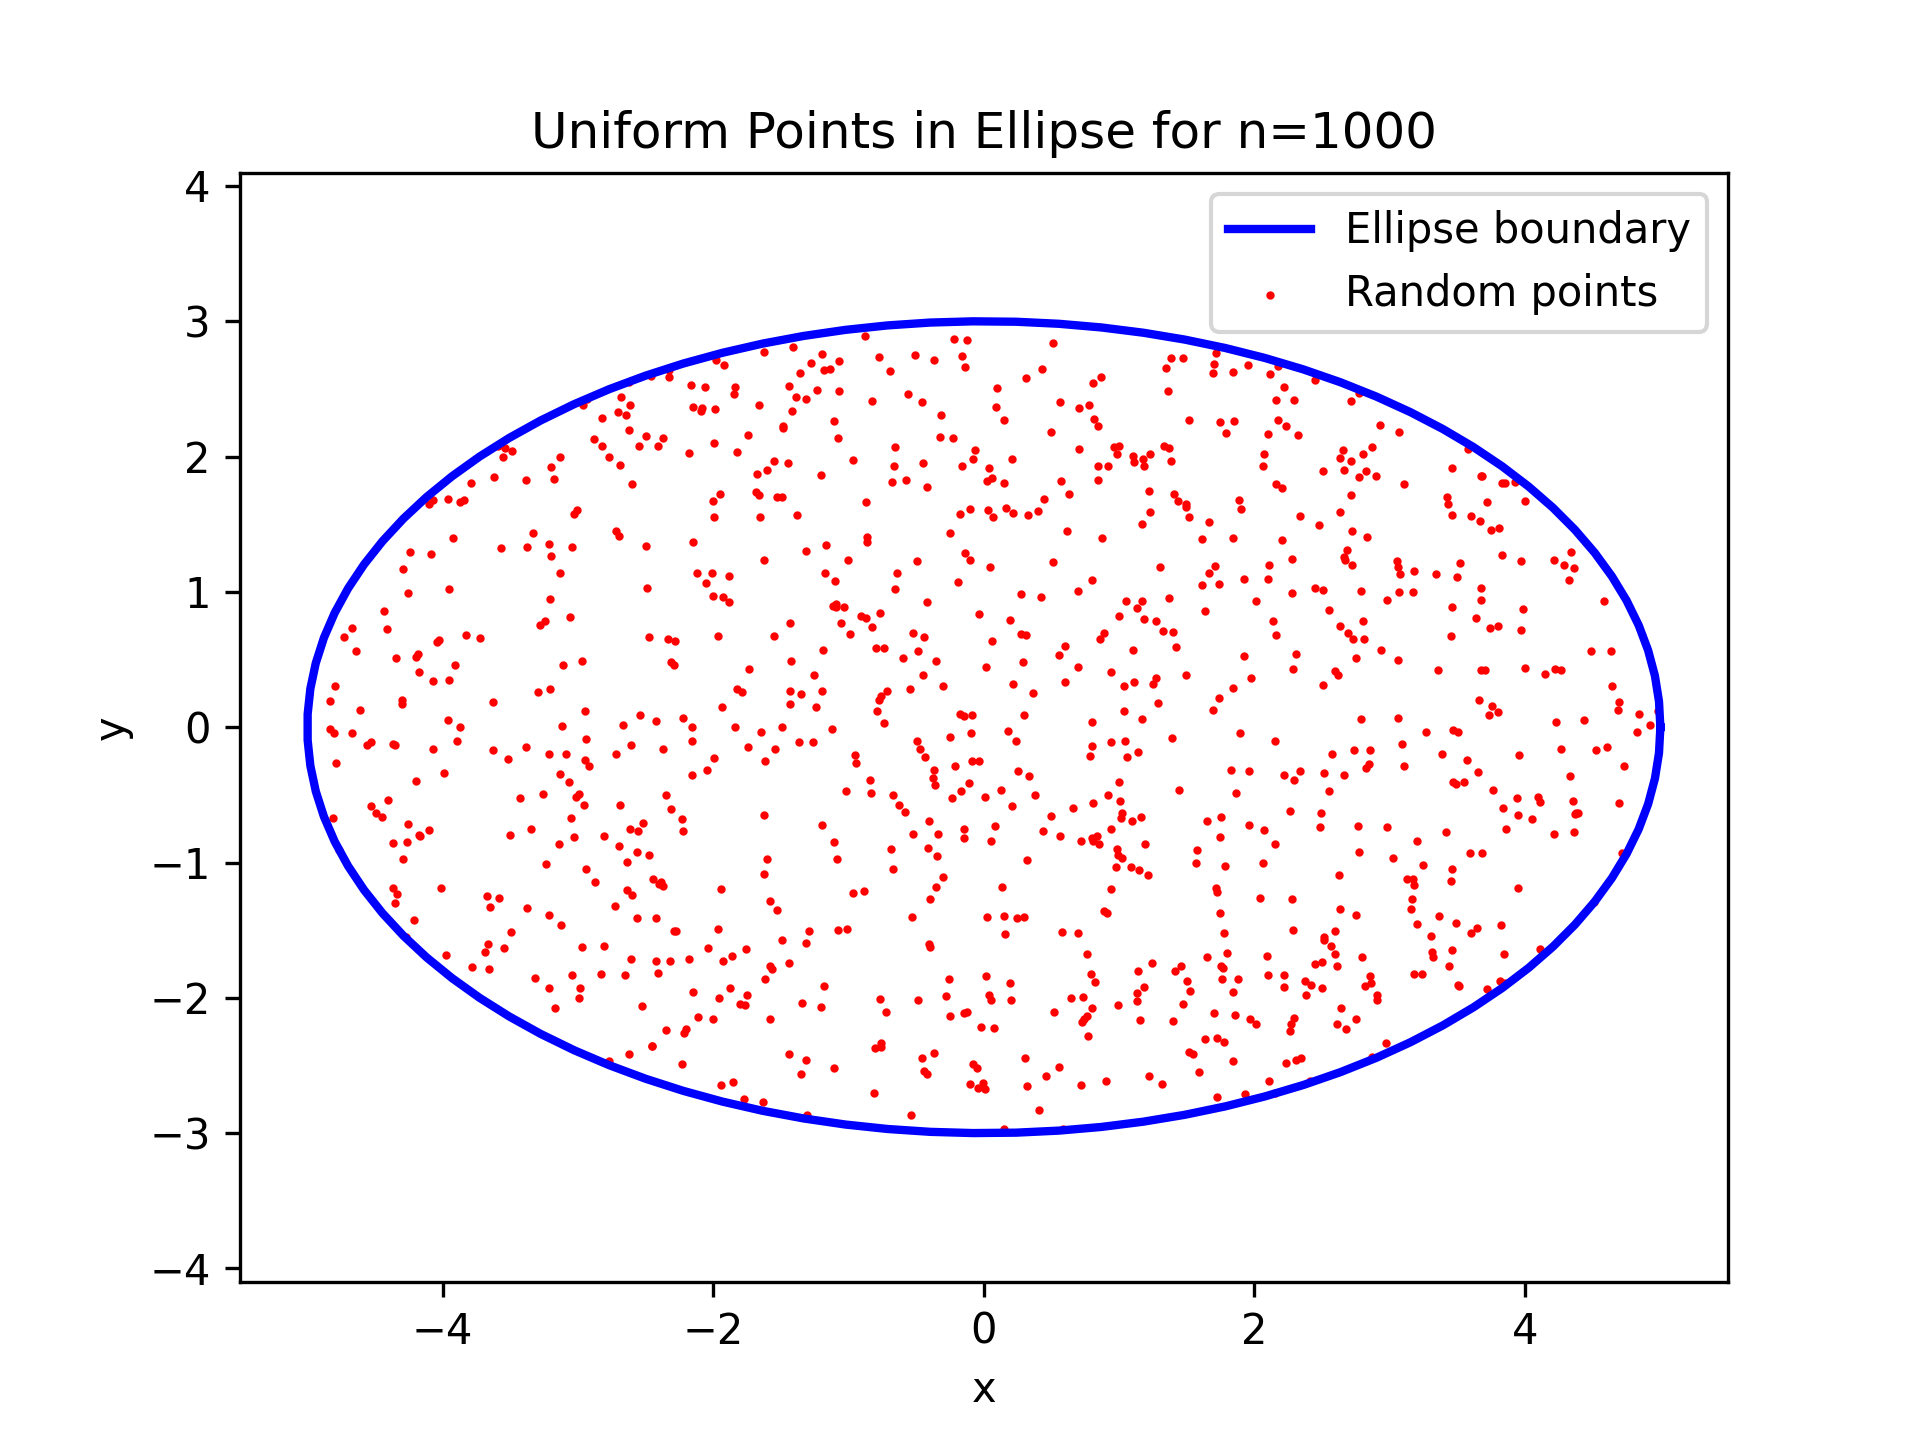
\includegraphics[width=\textwidth]{./Screenshots/Exercise5.2.png}
    \end{minipage}%
    \hfill
    \begin{minipage}{0.33\textwidth}
        \centering
        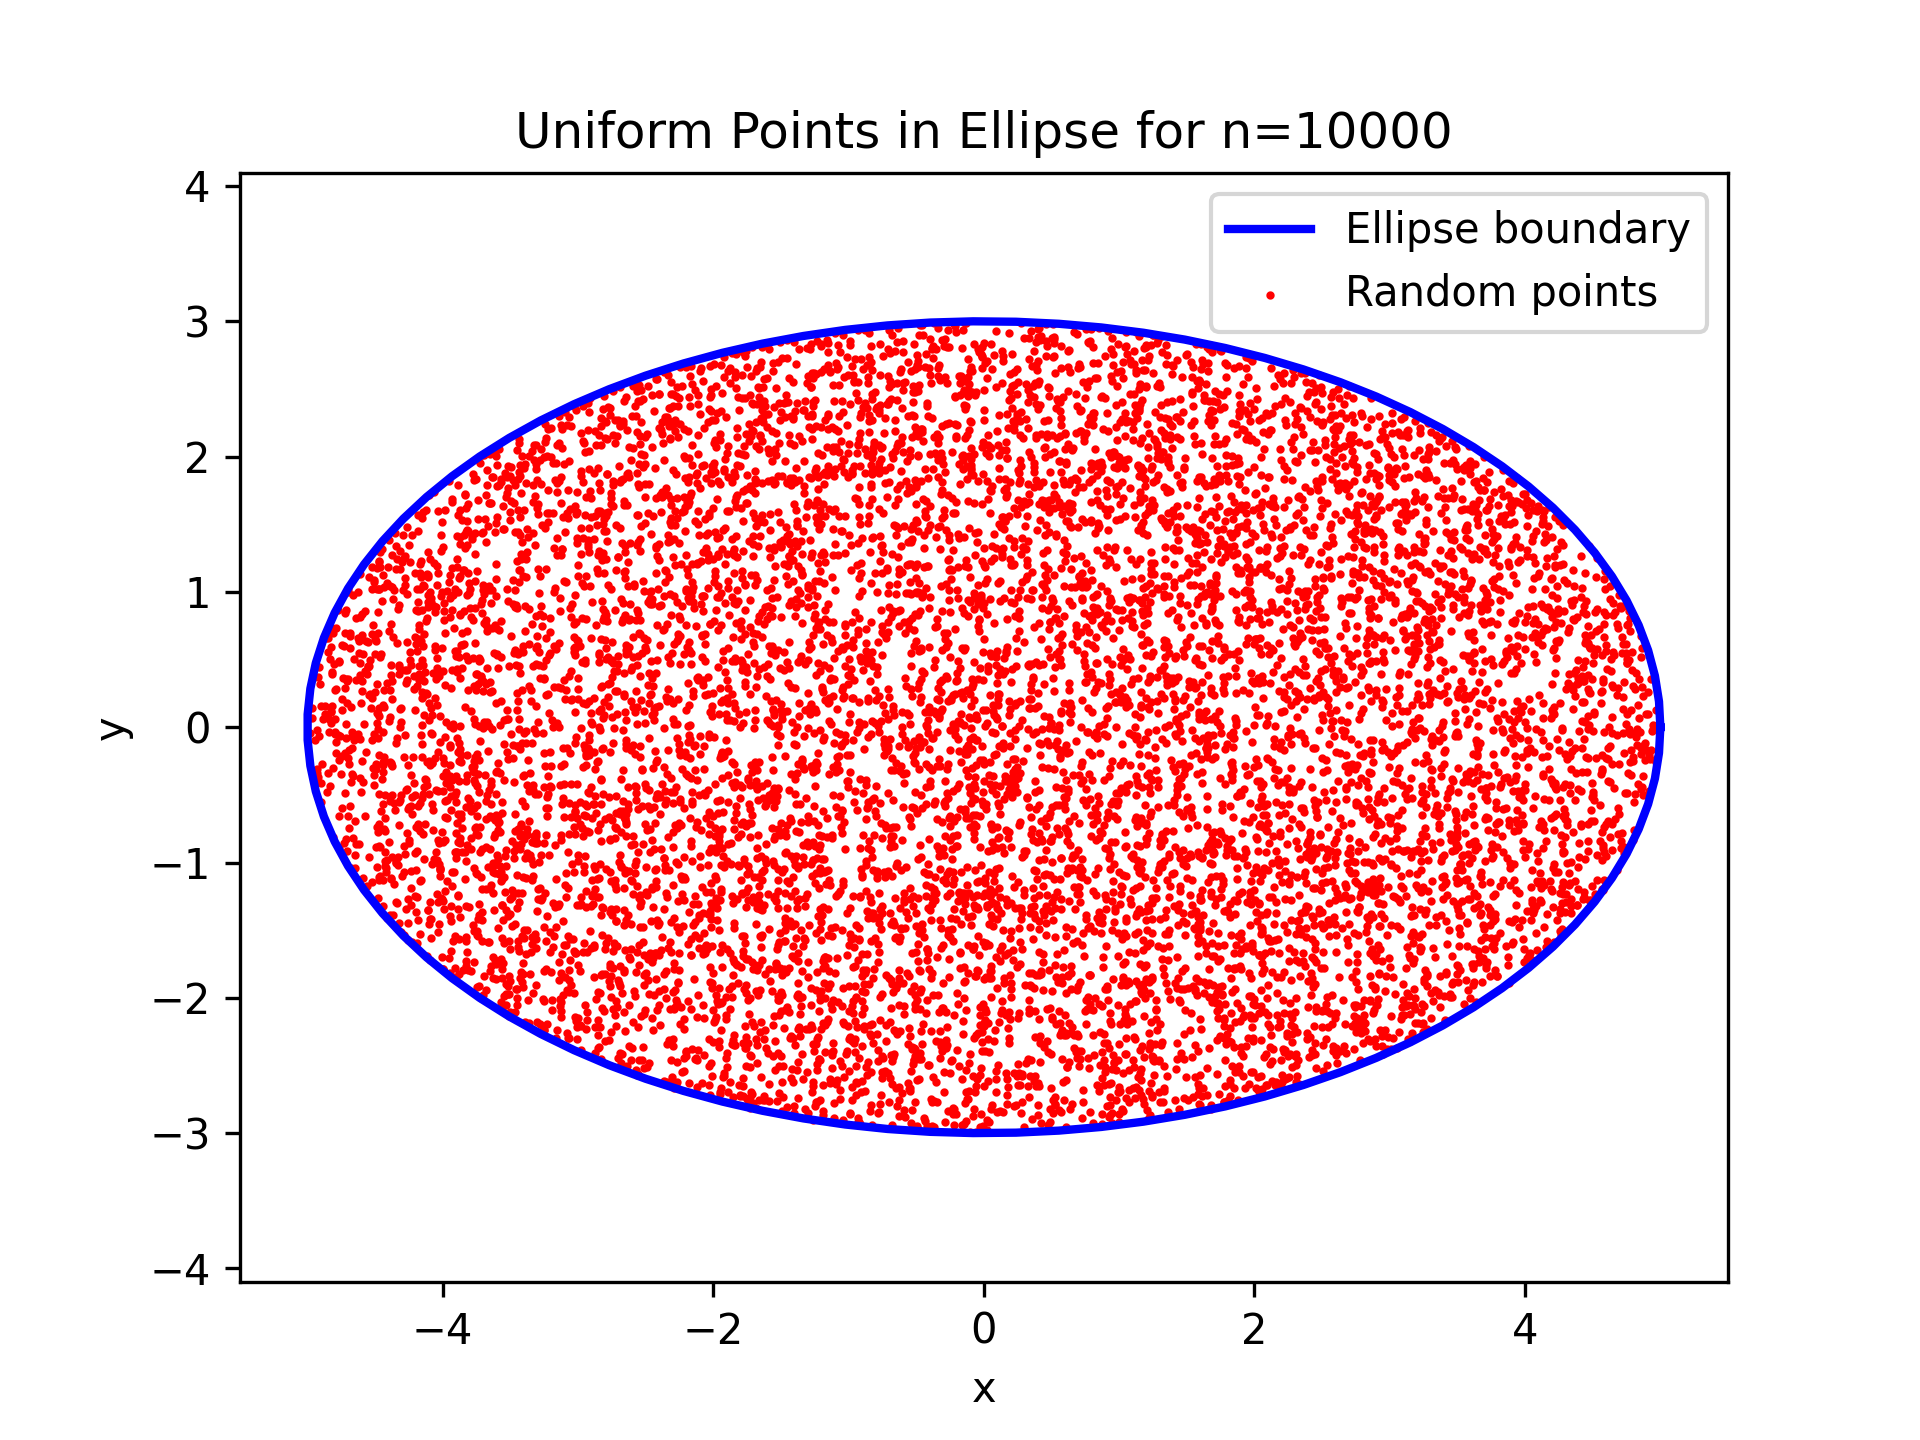
\includegraphics[width=\textwidth]{./Screenshots/Exercise5.3.png}
    \end{minipage}
\end{figure}
\newpage
\section{Exercise 6}
\begin{figure}[h!]
    \centering
    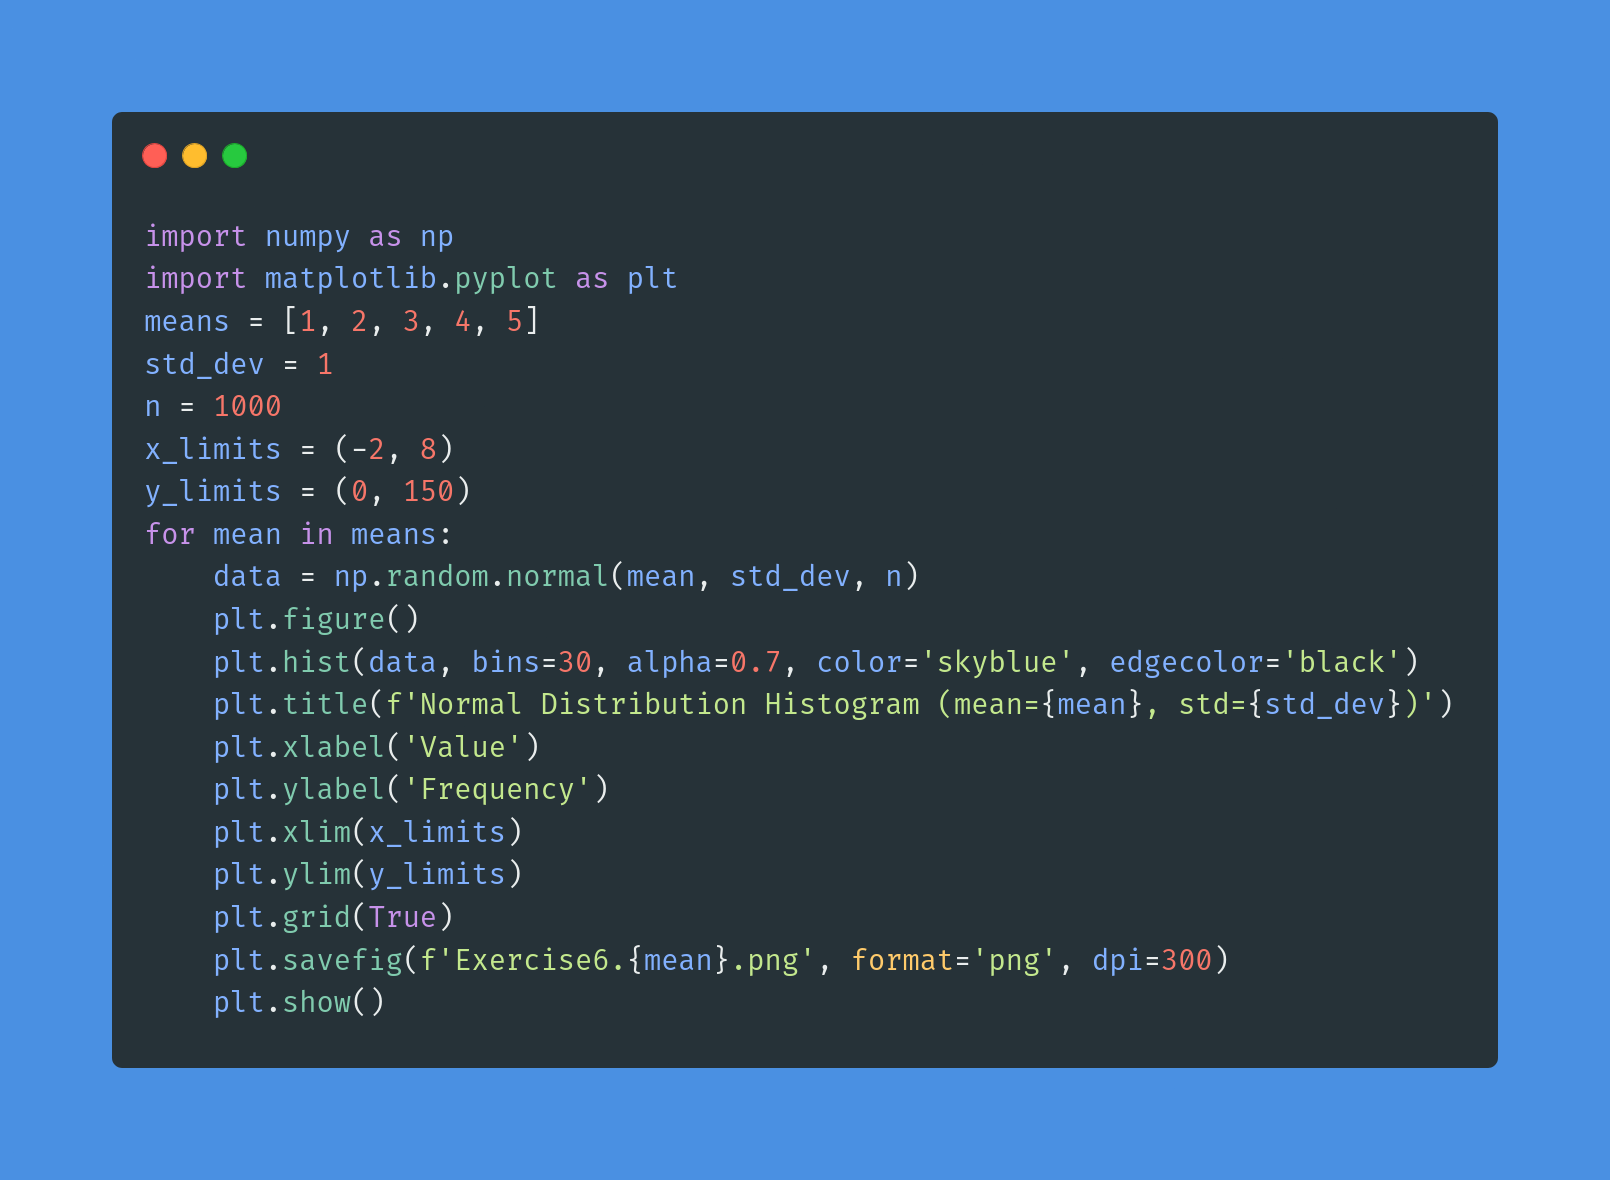
\includegraphics[width=0.8\textwidth]{./Screenshots/Exercise6.py.png} 
\end{figure} \\
\begin{figure}[h!]
    \centering
    \begin{minipage}{0.2\textwidth}
        \centering
        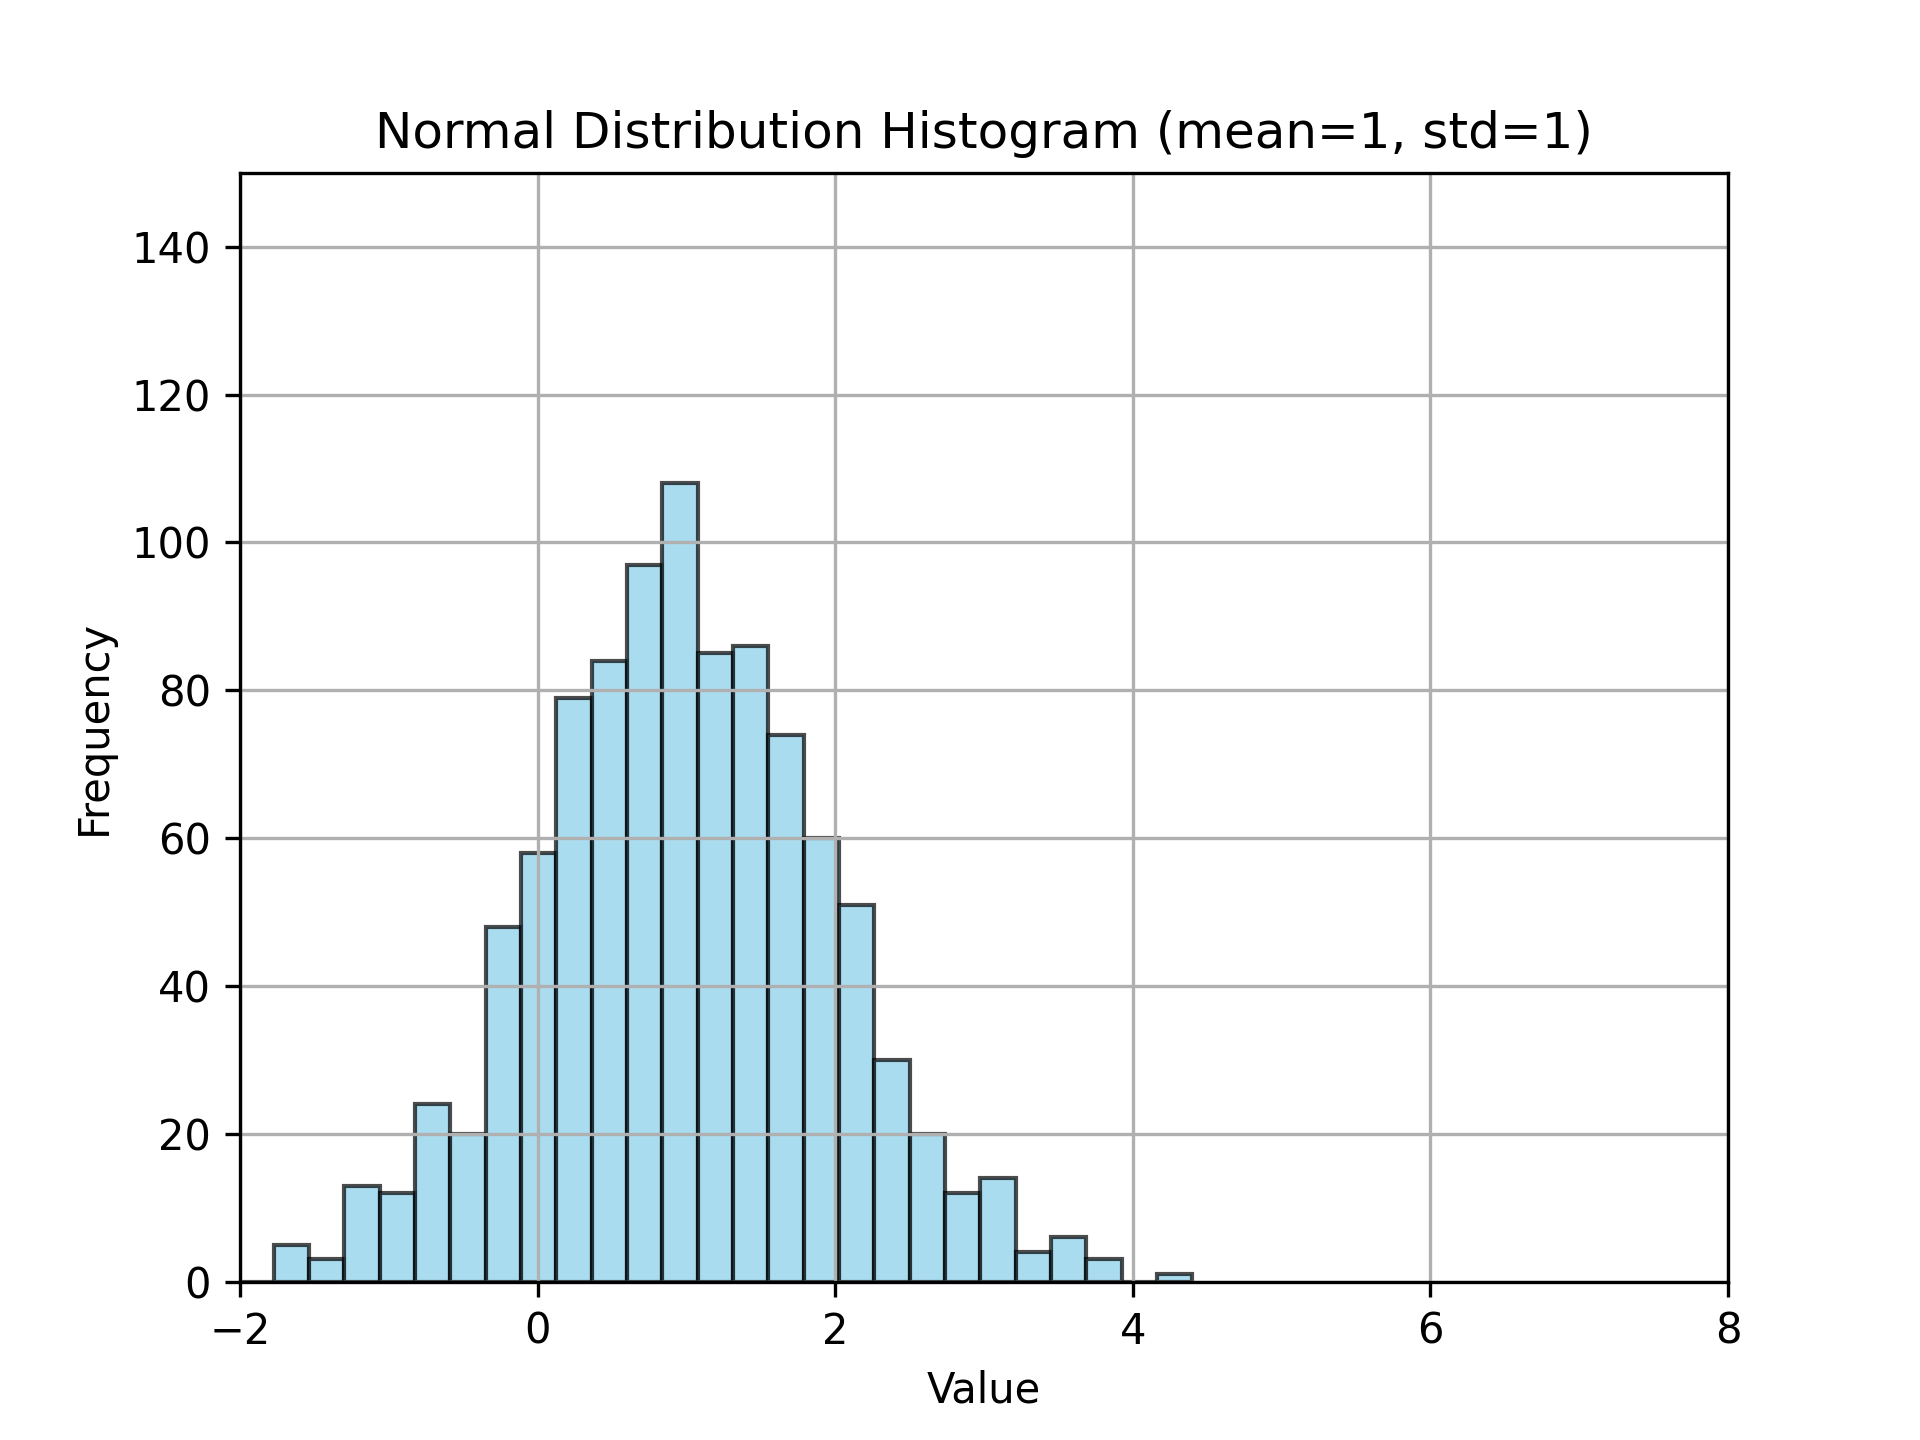
\includegraphics[width=\textwidth]{./Screenshots/Exercise6.1.png}
    \end{minipage}%
    \hfill
    \begin{minipage}{0.2\textwidth}
        \centering
        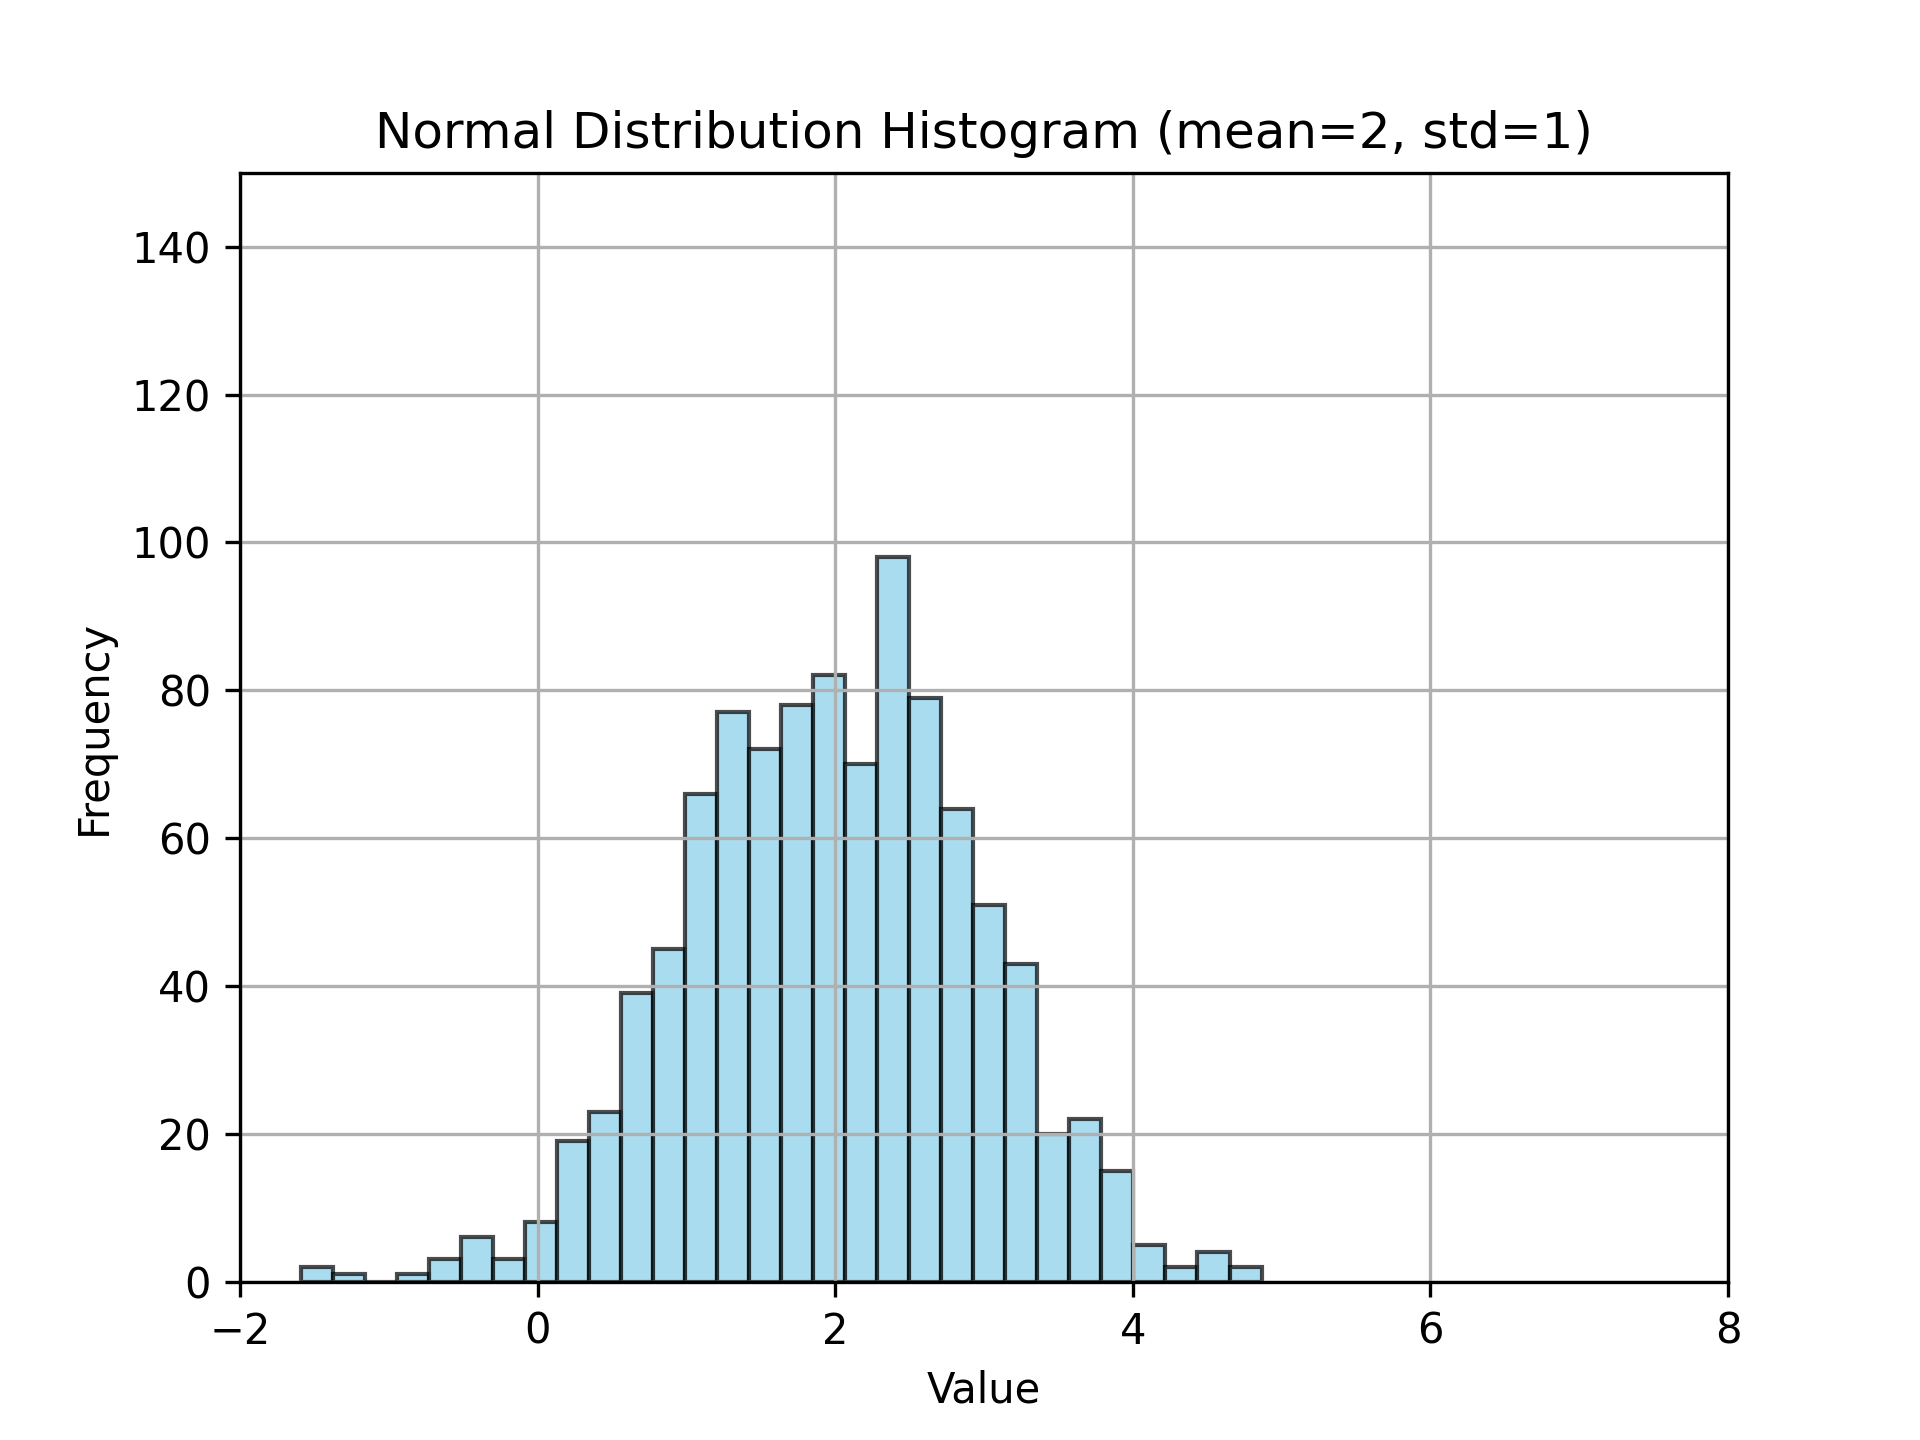
\includegraphics[width=\textwidth]{./Screenshots/Exercise6.2.png}
    \end{minipage}%
    \hfill
    \begin{minipage}{0.2\textwidth}
        \centering
        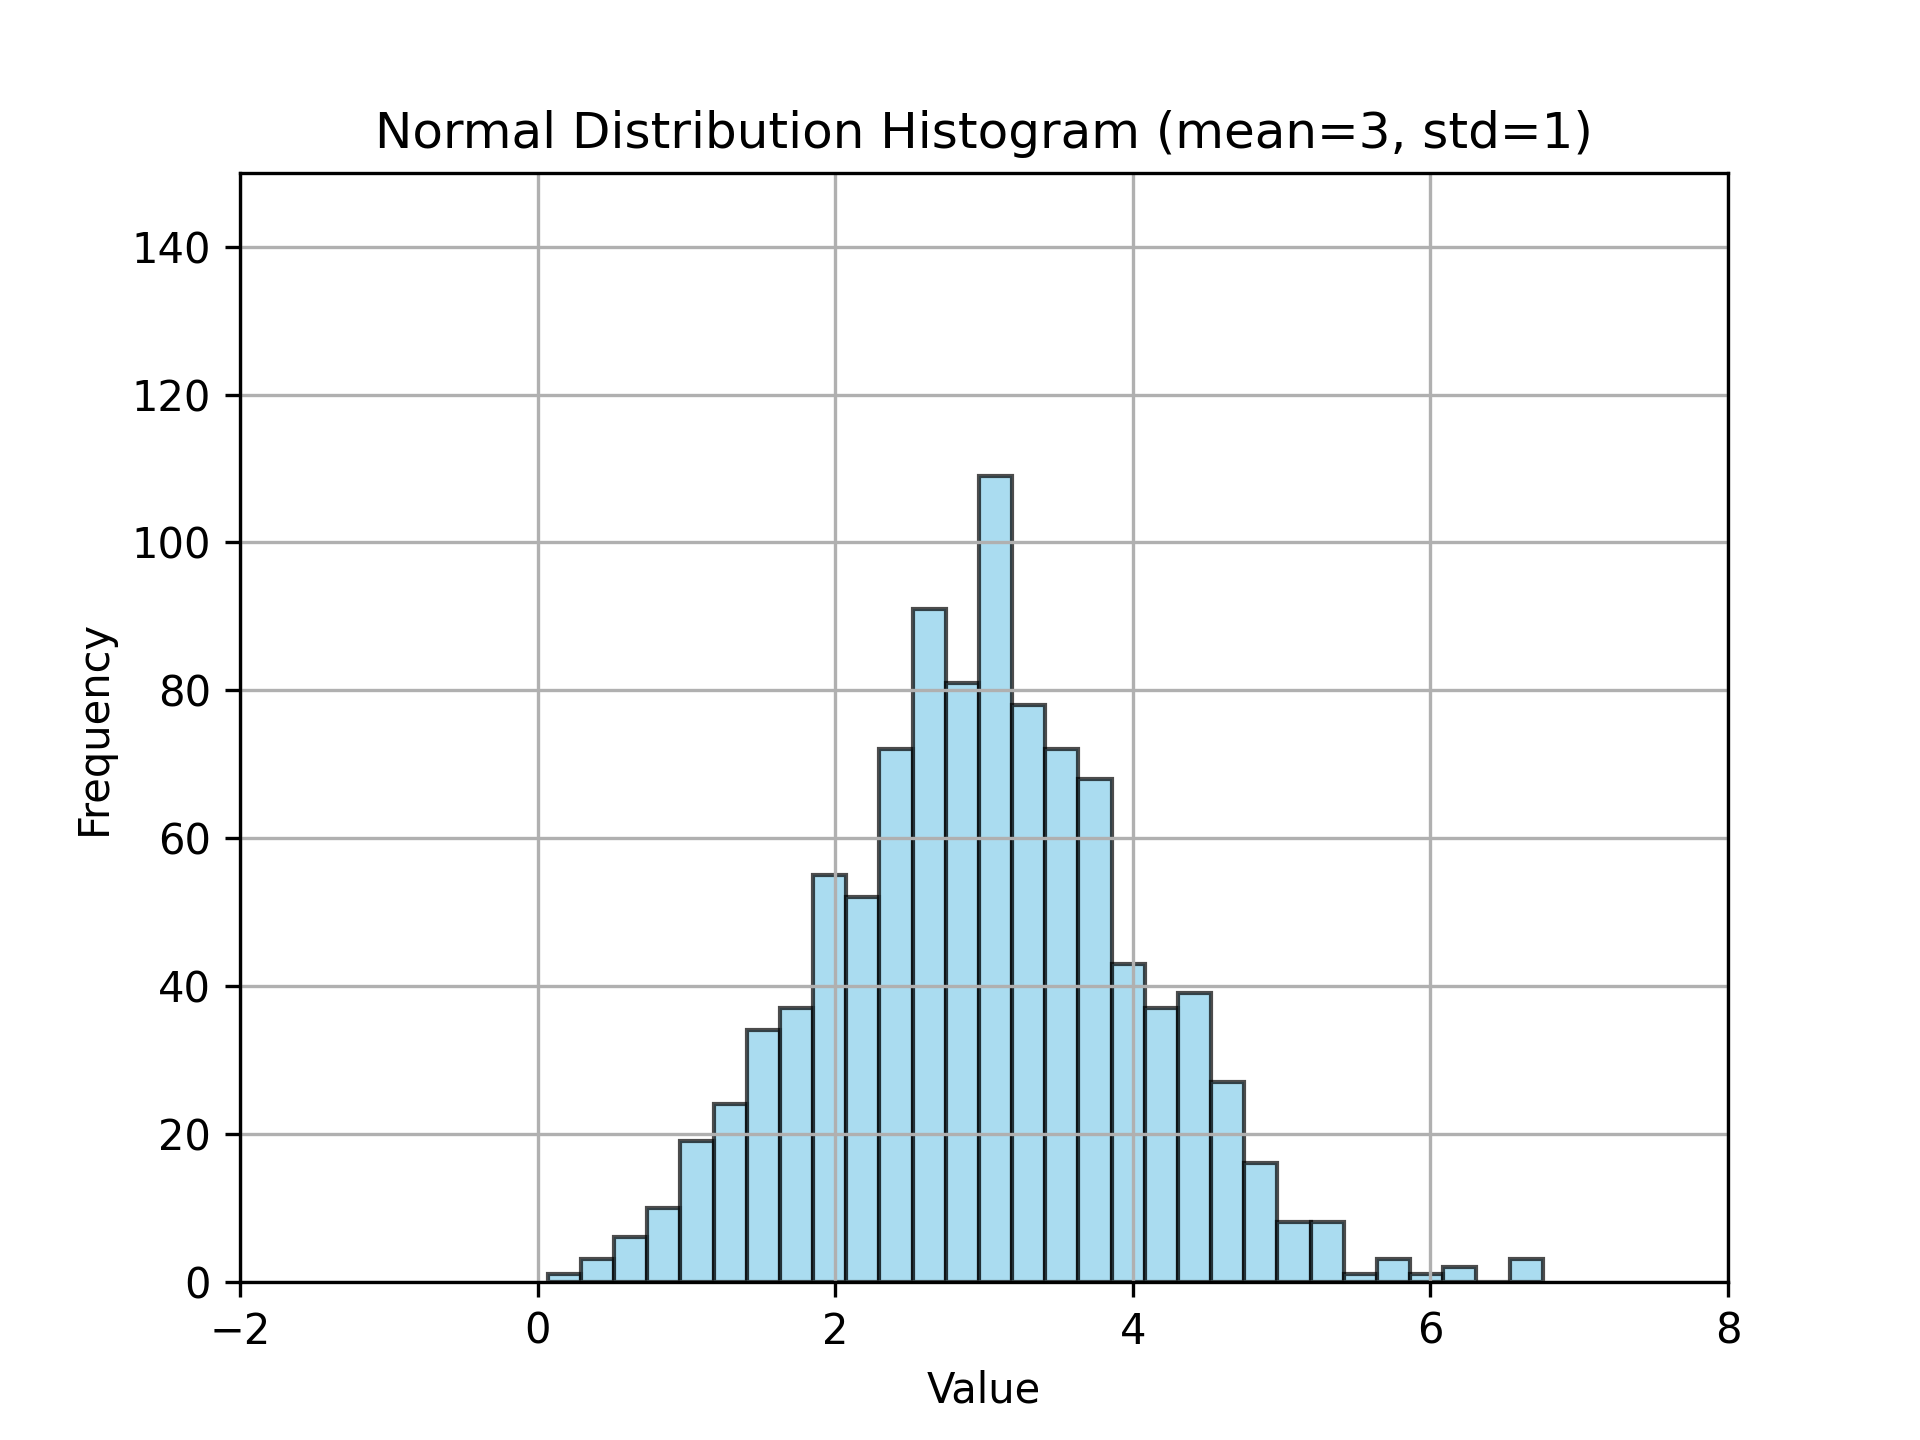
\includegraphics[width=\textwidth]{./Screenshots/Exercise6.3.png}
    \end{minipage}%
    \hfill
    \begin{minipage}{0.2\textwidth}
        \centering
        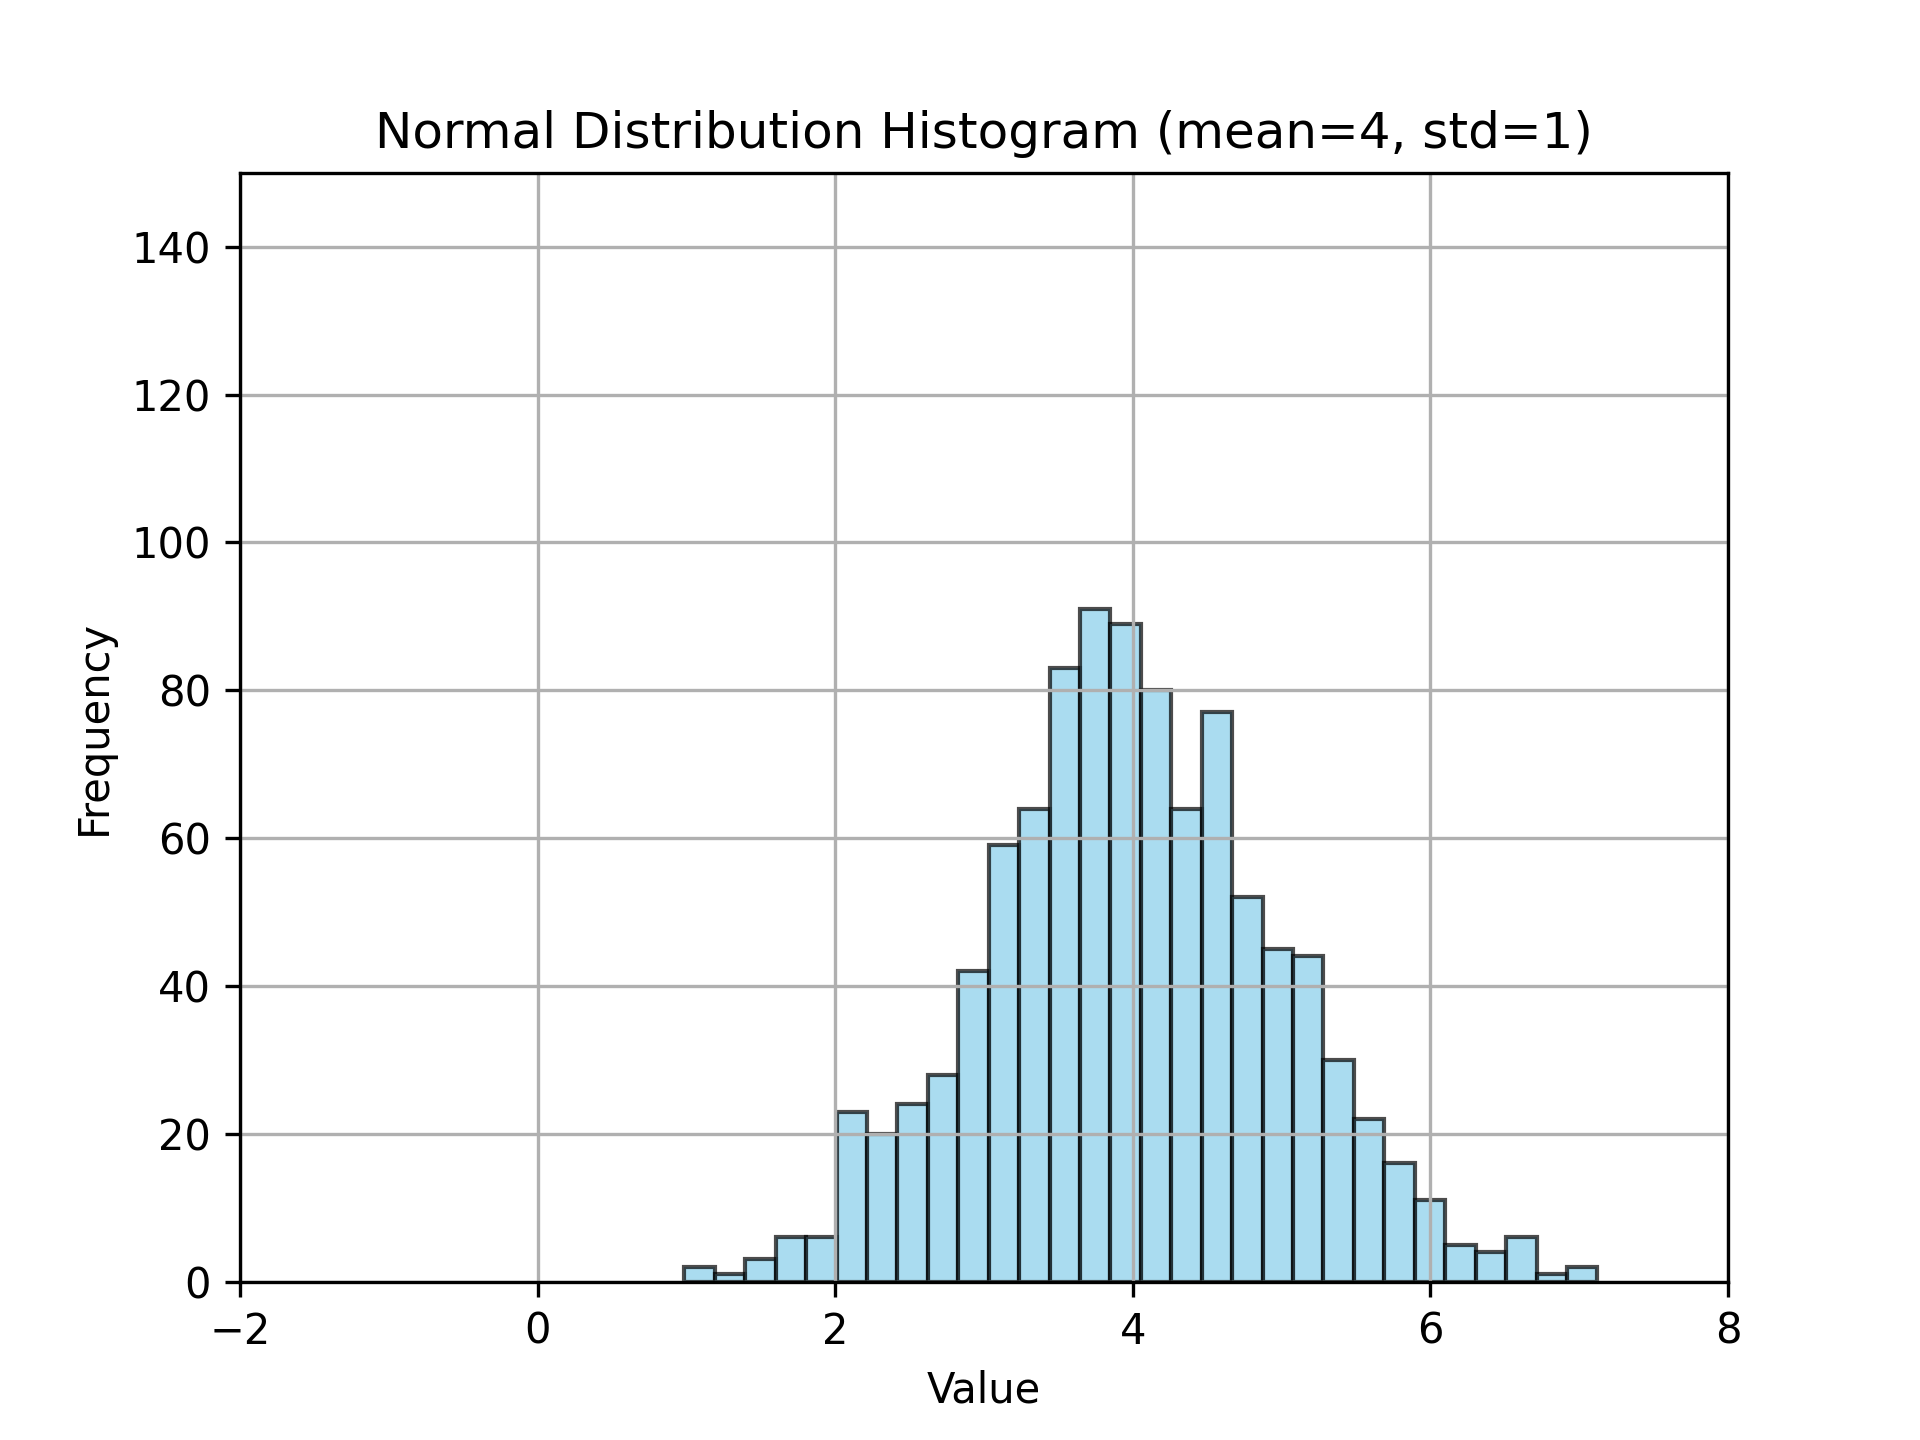
\includegraphics[width=\textwidth]{./Screenshots/Exercise6.4.png}
    \end{minipage}%
    \hfill
    \begin{minipage}{0.2\textwidth}
        \centering
        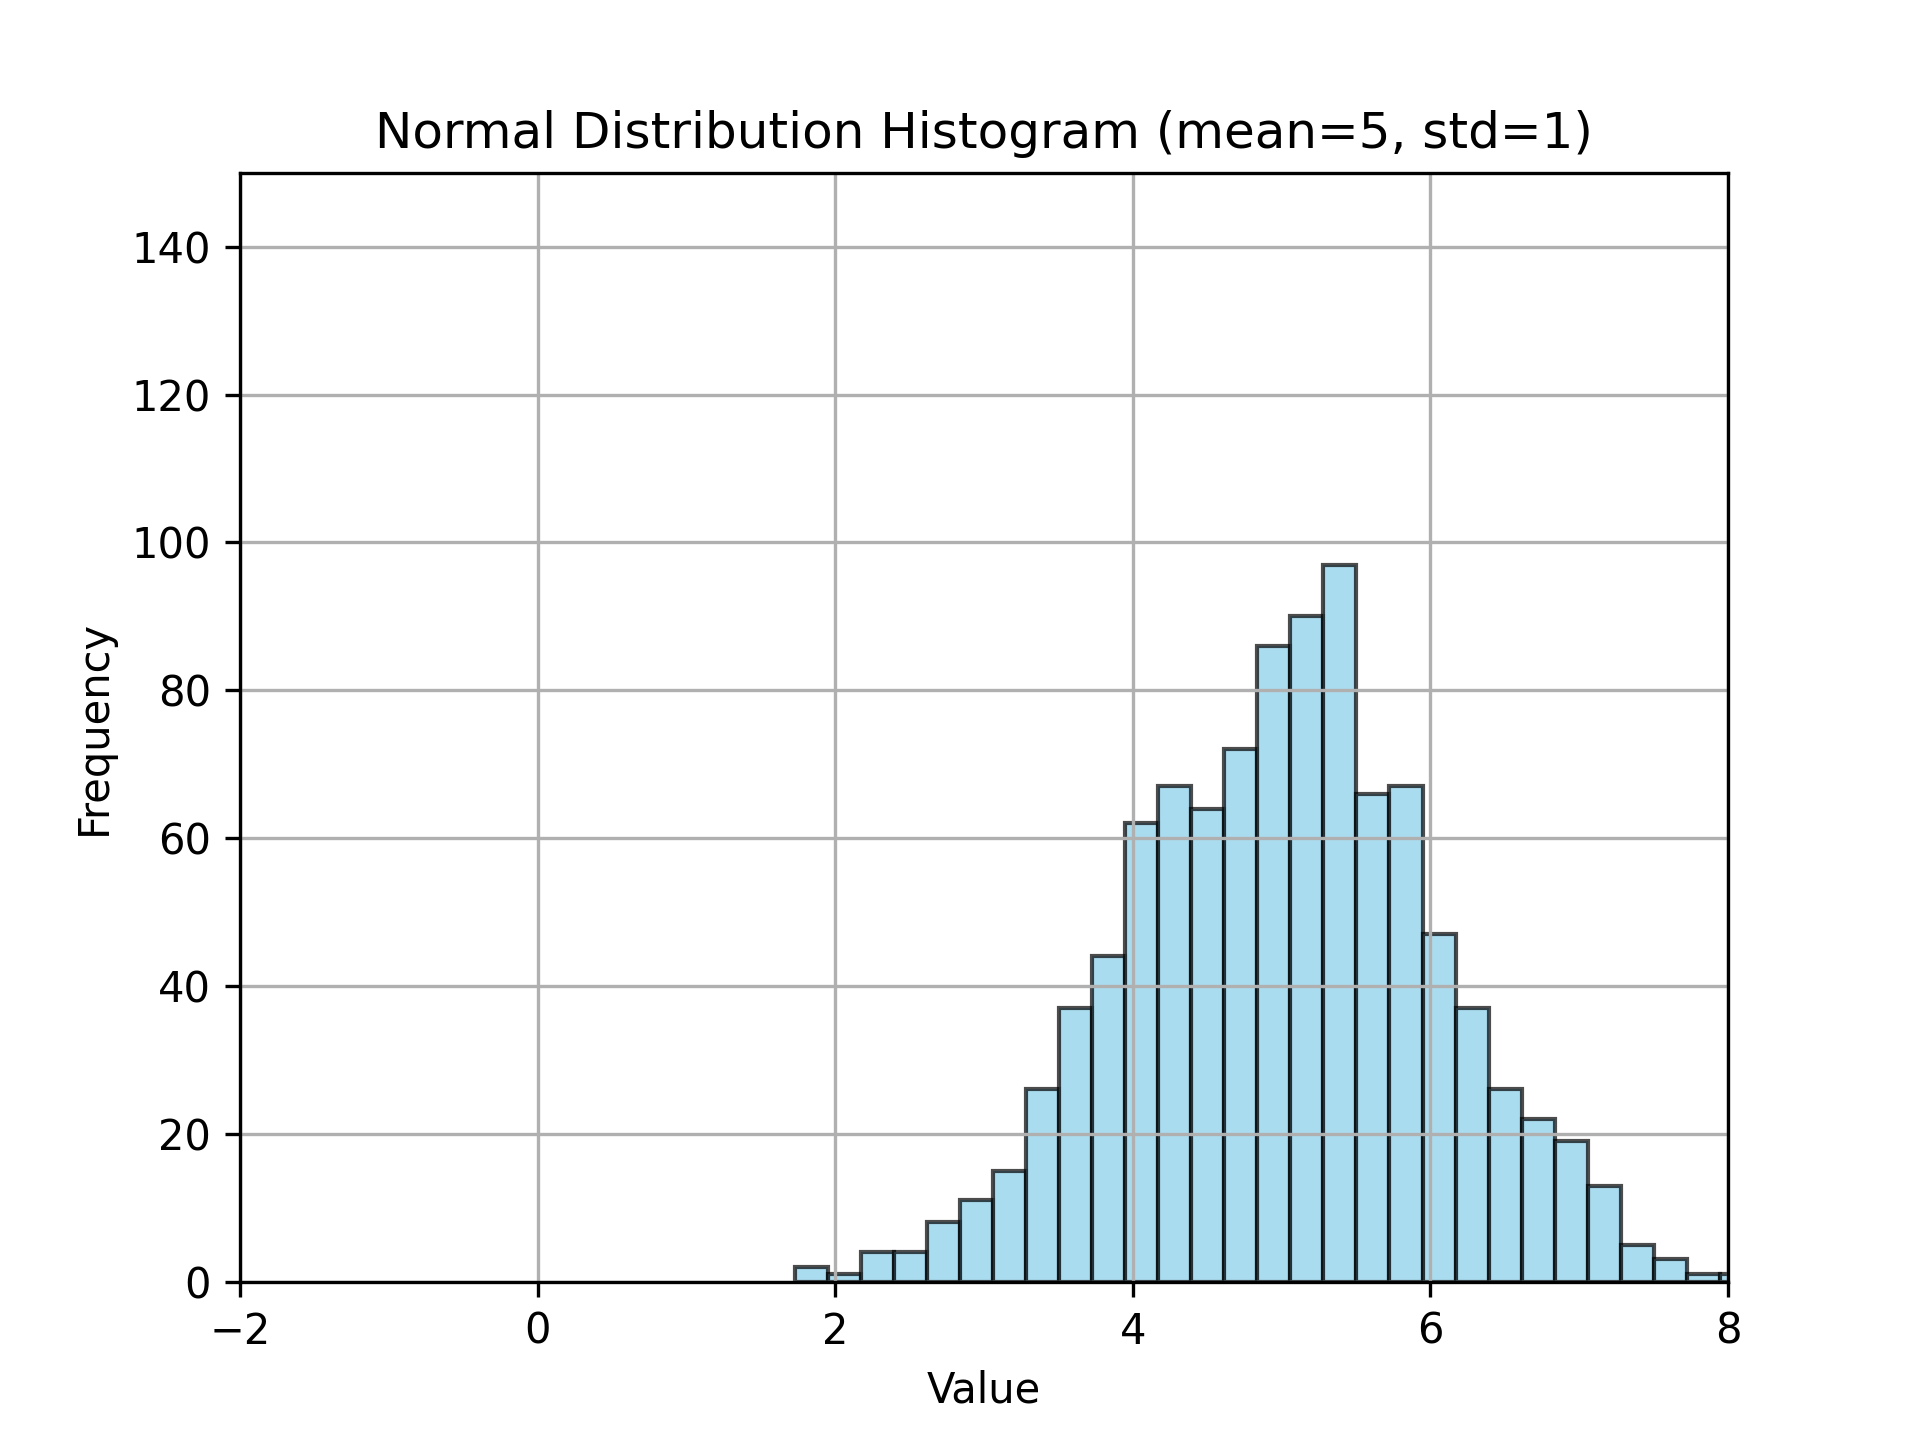
\includegraphics[width=\textwidth]{./Screenshots/Exercise6.5.png}
    \end{minipage}
\end{figure}
\newpage
\end{document}
